\documentclass[12]{article}

\usepackage{geometry}
\usepackage{amsmath, amsthm, amssymb}
\usepackage{graphicx}
\usepackage{tikz}
\usepackage{booktabs} % See the package documentation for guidelines on formal tables: https://ctan.org/pkg/booktabs
\usepackage{verbatim} % Used to typeset, for example, code snippets or pseudo-code for algorithms.
\usepackage{dsfont} % Extra fontset for helpful mathematics symbols, e.g. \mathds{1}
\usepackage{etoolbox} % Used to allow boolean variables for use in the title page
\usepackage{import}
\usepackage{lipsum}
\usepackage{subcaption}
\usepackage{float}
\usepackage{enumitem}
\usepackage{tabularx}
\usepackage{array}
\usepackage{pdfpages}
\usepackage{mathtools}
\usepackage{hyperref}
\usepackage{bbm}
\newcolumntype{C}[1]{>{\centering\arraybackslash}m{#1}}

\newcommand{\R}{\mathbb{R}}
\newcommand{\Q}{\mathbb{Q}}
\newcommand{\C}{\mathbb{C}}
\newcommand{\N}{\mathbb{N}}
\newcommand{\Z}{\mathbb{Z}}
\newcommand{\T}{\mathbb{T}}
\newcommand{\cA}{\mathcal{A}}
\newcommand{\cB}{\mathcal{B}}
\newcommand{\cD}{\mathcal{D}}
\newcommand{\cP}{\mathcal{P}}
\newcommand{\cM}{\mathcal{M}}
\newcommand{\abs}[1]{\left\lvert #1 \right\rvert}
\newcommand{\norm}[1]{\left\lVert #1 \right\rVert}
\newcommand{\set}[2]{\left\{#1 \ : \ #2\right\}}
\newcommand{\conv}[1]{\underset{#1}\longrightarrow}
\newcommand{\Mod}[1]{\ (\mathrm{mod}\ #1)}
\newcommand{\Supp}[0]{\ \mathrm{Supp}\ }
\DeclarePairedDelimiter\ceil{\lceil}{\rceil}
\DeclarePairedDelimiter\floor{\lfloor}{\rfloor}
\DeclareMathOperator{\lcm}{lcm}
\newcommand{\Cross}{\mathbin{\tikz [x=1.4ex,y=1.4ex,line width=.2ex] \draw (0,0) -- (1,1) (0,1) -- (1,0);}}

\newcommand\restr[2]{{% we make the whole thing an ordinary symbol
		\left.\kern-\nulldelimiterspace % automatically resize the bar with \right
		#1 % the function
		\vphantom{\big|} % pretend it's a little taller at normal size
		\right|_{#2} % this is the delimiter
}}
% Custom math operators (analogous to \lim, \sup, etc).
\DeclareMathOperator{\id}{id}
\DeclareMathOperator{\subspan}{span}
\DeclareMathOperator{\sgn}{sgn}
\DeclareMathOperator{\diam}{Diam}
\DeclareMathOperator{\mult}{mult}

\newtheorem{thm}{Theorem}[section] % Numbering is impacted by [chapter]; could do [section] or [subsection] also.
\newtheorem{lem}{Lemma} % The [thm] argument says to number Lemma in sequence with Theorem.
\newtheorem{prop}[thm]{Proposition}
\newtheorem{cor}[thm]{Corollary}
\newtheorem{conj}[thm]{Conjecture}
\newtheorem{question}{Question}
% These environments are unnumbered and will not count toward the numbering.
%\newtheorem*{question}{Question}
\newtheorem*{answer}{Answer}
\newtheorem*{conjecture}{Conjecture}
\newtheorem*{claim}{Claim}
% These environments are definitions; they have a different style (bold label, standard font).
\theoremstyle{definition}
\newtheorem{defn}[thm]{Definition} % These definitions are also numbered in sequence with Theorem.
\newtheorem{eg}{Example}
\newtheorem{rem}[thm]{Remark}
\newtheorem{obs}{Observation}

\title{ \vspace{-3cm} Ph.D. Working Notes }
%\author{Tao Gaede}

\begin{document}
	\maketitle
	\tableofcontents
	
	\section{Crescent Labelled Trees}
	
	Let $T$ be a tree of order $n$.  A crescent labelling of $T$ is a map $L: E(T) \mapsto \{1,2, \ldots, t\}$, such that the distance multiset of $L(T)$ is of the form $\{d_1^1,d_2^2, \ldots, d_{n-1}^{n-1}\}$.  The diameter of $T$, denoted $\diam(T)$, is the length of the $(u,v)$-path in $T$.  The max degree of $T$ is denoted $\Delta(T)$.  %We use $\ell$ to denote the number of leaves of $T$.
	

\begin{lem}[Basic Diameter Lower Bound]
	Let $t$ be a positive integer.  If $L(T)$ is a crescent labelling of the tree $T$ with weights $\{1,2,\ldots,t\}$, then $\diam(T) \geq \tfrac{n-1}{t}$.
\end{lem}

\begin{proof}
	Since there are at least $n-1$ distinct distances, there is a distance $d$ with value at least $n-1$.  Let $u,v \in V(T)$ such that $d(u,v) = d$, then since $t$ is the max edge weight, this means that the number of edges on a $(u,v)$-path is at least $\tfrac{d}{t} \geq \tfrac{n-1}{t}$.
\end{proof}
	
	
	For a pair of vertices $u,v \in V(T)$, we denote the $(u,v)$-path in $T$ as $P(u,v)$.  Lemma \ref{Lemma-DegreeClasses} below generalizes the observation underlying the maximum degree upper bound of $\sim$ $\sqrt{2n}$.
	
	\begin{lem}\label{Lemma-DegreeClasses}
		Let $T$ be a tree of order $n$.  For every $i \in [1,n-1]$, $M \in V(T)$, and $j \in \mathcal{N}(M)$, define
		$$D_j := \{u \in V(T) \setminus \{M\}: d(u,M) = d_i, j \in P(u,M)\}.$$
		Then distance $2d_i$ occurs with multiplicity at least $\sum_{j < k}^{\deg(M)} |D_j|\cdot |D_k|$.
	\end{lem}

	\begin{proof}
		Let $M \in V(T)$ and $i \in [1,n-1]$.  Since $T$ is a tree, there is always a unique $(u,v)$-path for all $u,v \in V(T)$.  So, for each $u \in D_j$ and $v \in D_k$, the $(u,v)$-path must go through $M$, which means $d(u,v) = d(u,M) + d(M,v) = 2d_i$.  There are $|D_j| \cdot |D_k|$ such $u$ and $v$ pairs, so indeed $2d_i$ has multiplicity at least $\sum_{j < k}^{\deg(M)} |D_j|\cdot |D_k|$. \qedhere
	\end{proof}
	
	Now we apply the lemma to get a condition on crescent labelled trees.
	
	\begin{prop}[Max Multiplicity Condition]
		Let $L(T)$ be a crescent labelling of a tree $T$.  Then for every $i \in [1,n-1]$, $M \in V(T)$, and $j \in \mathcal{N}(M)$, 
		$$\sum_{j < k}^{\deg(M)} |D_j|\cdot |D_k| < n.$$
	\end{prop}
	
	\begin{proof}
		Since $L(T)$ is a crescent labelling of $T$, no distance can have multiplicity greater than $n-1$and $T$ is a tree.  Since $T$ is a tree, it follows by Lemma \ref{Lemma-DegreeClasses} that for each vertex $M \in V(T)$, $i \in [1,n-1]$, $\sum_{j < k}^{\deg(M)} |D_j|\cdot |D_k| < n$. \qedhere
	\end{proof}
	
	Next is a general lemma on $\{1,2,\ldots,t\}$-words containing subwords with $t-1$ consecutive $1s$.
	
	\begin{lem}[Arithmetic Condition]\label{Lemma-ArithmeticCondition}
		Let $k \geq 2t$.  Let $\mathbf{w}$ be a $\{1,2,\ldots, t\}$-word with length $k$.  If $w_{a-t+2} = w_{a-t+3} = \cdots = w_{a} = 1$ for some $a \in \{1,2, \ldots, k\}$, then each value 
		$$1,2, \ldots, \max\biggr\{\sum_{i = 1}^{a}w_i, \sum_{i=a-t+2}^{k}w_i\biggr\}$$ 
		occurs as a partial sum in $\mathbf{w}$.
	\end{lem}
	
	\begin{proof}
		Suppose without loss of generality that $\sum_{i = 1}^{a}w_i \leq \sum_{i=a-t+2}^{k}w_i$.  Then it is sufficient to show that every value $1,2,\ldots, \sum_{i=a-t+2}^{k}w_i$ occurs as a partial sum in $\mathbf{w}$.  Call $w_{a-t+2},w_{a-t+3}, \ldots, w_a$ the \emph{unit segment} of $\mathbf{w}$ and $w_{a+1},w_{a+2},\ldots,w_k$ the \emph{non-unit segment} of $\mathbf{w}$.  We proceed by induction on the number of terms $r$ in the non-unit segment of $\mathbf{w}$.  When $r = 1$, $w_{a+r} \in \{1,\ldots,t\}$, and since the unit segment has $t-1$ 1s, for each $j \in \{1,2,\ldots,t-1\}$, we have the partial sums $j = \sum_{i=0}^{j-1}w_{a-i}$.  Then the values between $w_{a+r}$ and $\sum_{i=a-t+2}^{a+r}w_i$ are of the form $w_{a+r}+ \sum_{i=0}^{j-1}w_{a-i}$.  For the inductive step, the values $1,2,\ldots,\sum_{i=a-t+2}^{a+r-1}w_i$ occur at least once by inductive hypothesis.  We have that $w_{a+r} \in \{1,2,\ldots,t\}$ and the values between $\sum_{i=a+1}^{a+r-1}w_i$ and $\sum_{i=a+1}^{a+r}w_i$ can be obtained from $\sum_{i=a+1-j}^{a+r-1}w_i$ for each $j \in \{1,2,\ldots,t-1\}$.  Then similarly the values between $\sum_{i=a+1}^{a+r}w_i$ and $\sum_{i=a-t+2}^{a+r}w_i$ are $\sum_{i=a+1-j}^{a+r}w_i$ for $j \in \{1,2,\ldots,t-1\}$. \qedhere
	\end{proof}
	
	We now apply this arithmetic lemma to crescent labelled trees to show that when there are many consecutive 1s on a path, the path cannot be too long with many large weight edges.
	
	\begin{prop}
		Let $L(T)$ be a crescent labelling of a tree $T$ with edge weights in $\{1,2,\ldots,t\}$.  Then for every path $P = (v_1v_2,v_2v_3,\ldots,v_{t-1}v_t)$ in $T$ such that $w(v_iv_{i+1}) = 1$ for $i \in \{1,2,\ldots,t-1\}$, it follows that $\max\{d(v_1,u): u \in V(T)\} < n$ and $\max\{d(v_t,u): u \in V(T)\} < n$.
	\end{prop}
	
	\begin{proof}
		Let $T$ be a tree with a path $P$ specified in the proposition statement and $L(T)$ a crescent labelling.  It is sufficient to show that $\max\{d(v_1,u): u \in V(T)\} < n$ since the case for $v_t$ is similar.  Let $u' \in V(T)$ such that $d(v_1,u') = \max\{d(v_1,u): u \in V(T)\}$.  By Lemma \ref{Lemma-ArithmeticCondition}, every distance $1,2,\ldots, d(v_1,u')$ occurs at least once.  Since $L(T)$ is a crescent labelling, there can be at most $n-1$ distinct distances, so $d(v_1,u') < n$ as desired. \qedhere
	\end{proof}
	The implication for when $t=2$ is quite strong since this imposes a max distance condition on vertices incident to edges with weight $1$.
	\begin{cor}
		Let $L(T)$ be a crescent labelling of a tree $T$.  If $t = 2$, then every vertex incident to an edge with weight $1$ has max distance at most $n-1$.
	\end{cor}
	
	%\begin{prop}
	%	Let $L(T)$ be a crescent labelling of a tree $T$.  For every path $P$ of length $t-1$ whose edges all have weight $1$, each end vertex $v \in P$ satisfies 
	%	$$\max\{d(v,u):u \in V(T)\} \leq n.$$
	%\end{prop}
	
	What follows is a basic lemma about trees that may turn out to be useful in case parameterizing by number of leaves becomes sensible.
	
	\begin{lem}[From Chartrand and Lesniak's text ``Graphs and Digraphs" 4th edition]
		Let $T$ be a tree with $n_i$ vertices with degree $i$, where $i \in \{1,2,\ldots,\Delta(T)\}$.  Then $n_1 = n_3 + 2n_4 + 3n_5 + \cdots + (\Delta(T)-2)n_{\Delta(T)} + 2$.
	\end{lem}
	
	\begin{proof}
		Note that $n = \sum_{i=1}^{\Delta(T)}n_i$.  Since $T$ is a tree, 
		$$\sum_{i=1}^{\Delta(T)} in_i  = \sum_{v \in V(T)} \deg(v) = 2(n-1) = 2\biggr(\sum_{i=1}^{\Delta(T)}n_i \biggr) - 2.$$  
		Rearranging gives $2+ \sum_{i=1}^{\Delta(T)} (i-2)n_i = 0.$
	\end{proof}
	
	\begin{cor}
		If $T$ is a tree, then $\sum_{i=3}^{\Delta(T)}(i-2)n_i < n_1$
	\end{cor}
	
	\section{Polynomial Method}
	
	Let $L(G)$ be a crescent labelling of a graph $G$ with corresponding distance multiset $\{d_1^{1},d_2^{2},\ldots,d_{n-1}^{n-1}\}$. Consider the bipartite multigraph $\mathcal{M} := \mathcal{M}(G)$ where $V(\mathcal{M}) = X \cup Y$, where $X$ consists of the distinct distances $d_1,d_2,\ldots,d_{n-1}$ and $Y$ consists of the vertices of $G$, $v_1,v_2,\ldots,v_n$.  For $d_k\in X$ and $v_i \in Y$, an edge $d_kv_i \in E(\mathcal{M})$ is included for every $j \in [n]$ such that $d(v_i,v_j) = d_k$.  Note that since $L(G)$ is a crescent labelling, for each $k \in [n-1]$, $\deg(d_k) = 2k$.  Observe also that the multiset neighbourhood of $v_i$ is the multiset of the $n-1$ distances between $v_i$ and the other vertices in $G$.
		
	We show a variation of a result from Alon (see proof of Theorem 6.1 in \cite{alon}) about the existence of $p$-regular subgraphs of a multigraph whose average degree is very close to its max degree.  If we relax this strong average degree condition, we can still obtain a rather powerful result whereby a subgraph $U$ of $\mathcal{M}$ has vertex degrees in $\{p,2p,3p,4p,5p,6p,7p\} \cap [2(n-1)]$, where $p \in [\tfrac{n}{4},\tfrac{n}{2}]$, which is significant because $\mathcal{M}$ is bipartite and so the structure of $U$ can tell us some things about how the distances relate to the vertices in $G$.  This subgraph $U$ likely can't be too small, since then there would be a vertex $v \in G$ with too many other vertices at some distance $d$ from $v$.  
	
	\begin{rem}
		Relating the size of this $U$ to the structure of $G$ might be a fruitful way to proceed.  For instance, paths require $|U|$ to be quite large (no vertex is at distance $d$ with more than $2$ other vertices for each $d$).  I think stars might be similar in that they require $|U|$ to be rather large.  Perhaps if $p \sim n/4$, or even asymptotically when $p \sim n/2 - (n/2)^{0.525}$ or so, $U$ being large with min degree $p$ forces convergence of crescent labelled trees to paths and stars.  But I admit, I'm not really sure right now what to do when $|U|$ is big.
	\end{rem}
	
	
	%The key result here is Corollary XX, which says that any crescent labelled graph forces at least one of the vertices to be at distance $d$ from at least $p$ other vertices, where $p \in [\tfrac{n}{4}, \tfrac{n}{2}]$.  
	
	The proof applies Alon's combinatorial nullstellensatz \cite{alon}.  The corollary of the nullstellensatz that we use is as follows:
	
	\begin{lem}[Combinatorial Nullstellensatz]\label{Lemma-CombinatorialNullstellensatz}
		Let $\mathbb{F}$ be a field and let $f \in \mathbb{F}[x_1,x_2,\ldots,x_n]$ be a polynomial such that $\deg(f) = \sum_{i=1}^n t_i$ and the coefficient of $\prod_{i=1}^n x_i^{t_i}$ is non-zero.  Let $S_1,S_2,\ldots,S_n$ be subsets of $\mathbb{F}$ such that $|S_i| > t_i$ for all $i \in [n]$.  Then there exists $(s_1,s_2,\ldots,s_n) \in S_1 \times S_2 \times \cdots \times S_n$ such that $f(s_1,s_2,\ldots,s_n) \neq 0$.
	\end{lem}
	
	\begin{prop}[Variation of Theorem 6.1 in \cite{alon}]\label{Prop-SubgraphNullstellensatzResult}
		Let $p$ be a prime number in $[\tfrac{n}{4},\tfrac{n}{2}]$.  Then $\mathcal{M}(G)$ contains a subgraph $U$ such that for every $u \in V(U)$, $\deg(u) \in \{p,2p, 3p,4p,5p,6p,7p\} \cap [2(n-1)]$.  %In particular, $U$ contains vertices in each part of $\mathcal{M}$, each with degree at least $p$.
	\end{prop}
	\begin{proof}
		We define a polynomial $f$ with degree $|E(\mathcal{M})|$ over $\mathbb{F}_2$, and using the fact that $a^{p-1}$ $\Mod{p}$ $\equiv 1$ for all $a \not\equiv 0 \Mod{p}$, we show the existence of the desired subgraph using the nullstellensatz directly.
		
		Define the polynomial
		$$f(x_e:e \in E(\mathcal{M})) = \prod_{v \in V(\mathcal{M})} \biggr[1 - \Big(\sum_{\substack{e \in E(\mathcal{M})\\ v \in e}}x_e \Big)^{p-1} \biggr] - \prod_{e \in E(\mathcal{M})}(1-x_e).$$
		
		The degree of $f$ is $|E(\mathcal{M})|$ because
		$$|V(\mathcal{M})| (p-1) = (2n-1)(p-1) \leq (2n-1)(\tfrac{n}{2}-1) = n(n-\tfrac{5}{2})+1 < n(n-1) = |E(\mathcal{M})|.$$
		
		Note that the max degree term, $(-1)^{|E(\mathcal{M})|}\prod_{e \in E(\mathcal{M})} x_e$ has a non-zero coefficient. 
		To apply the nullstellensatz, we consider solutions to $f$ of the form $(s_1,s_2,\ldots,s_{|E(\mathcal{M})|}) \in \{0,1\}^{|E(\mathcal{M})|}$ (where $t_i = 1$ for all $i \in [|E(\mathcal{M})|]$).  Thus by Lemma \ref{Lemma-CombinatorialNullstellensatz}, there exists a vector, call it $r=(r_e:e \in E(\mathcal{M}))$, such that $f(r) \neq 0$.  By the definition of $f$, $r \neq 0$ because $f(0) = 0$, so some of its entries are $1$.  This means that the latter product in $f$ vanishes when evaluated at $r$.  The former product in $f$ can be non-zero only when $\Big(\sum_{\substack{e \in E(\mathcal{M})\\ v \in e}}r_e \Big)^{p-1} \equiv 0 \Mod{p}$.  It follows that $r$ corresponds to a subgraph $U$ of $\mathcal{M}(G)$ whose vertex degrees are congruent to $0 \Mod{p}$.  Since $\Delta(\mathcal{M}) = 2(n-1)$ and $r \neq 0$, there exists a vertex $u \in U$ such that $\deg(u) \in \{p,2p, 3p, 4p, 5p, 6p, 7p\} \cap [2(n-1)]$.  Note that since the degrees of the vertices in the neighbourhood of $u$ are all at least $1$, $U$ contains at least one vertex in each part of $\mathcal{M}$ with degree at least $p$. \qedhere
	\end{proof}

	%\begin{cor}
	%	Let $L(G)$ be a crescent labelling of a graph $G$ and $p$ be a prime number in $[\tfrac{n}{4}, \tfrac{n}{2}]$.  Then there exists a vertex $v \in V(G)$ and a distance $d \in \{d_1,d_2,\ldots,d_{n-1}\}$ such that there are at least $p$ other vertices in $G$ at distance $d$ from $v$.
	%\end{cor}
	
	\section{Distance Multiplicities in Unweighted Graphs}
	
	Let $G$ be a tree. Define $T(G)$ to be $G$ without its leaves, and on each vertex $v$ of $T(G)$ assign it a weight equal to the degree of $v$ in $G$, $\deg(v)$.  Define $m(k)$ to be the multiplicity of distance $k$ in a graph $G$.
	
	The following expresses $m(k)$ in terms of the degrees of the vertices of $G$, or equivalently, the vertex weights in $T(G)$.
	
	\begin{lem}[Characterizing Distance Multiplicities in Terms of Vertex Degrees]\label{Lemma-CharacterizingMultiplicityInTermsOfDegrees}
		It holds that $m(1) = |E(G)|$, $m(2) = \sum_{v \in V(G)} {\deg(v) \choose 2}$, and when $3 \leq k \leq \diam(G)$, 
		$$m(k) = \sum_{\substack{\{x,y\} \subset T(G) \\ d(x,y) = k-2}} (\deg(x)-1)(\deg(y)-1).$$
	\end{lem}

	\begin{proof}[Proof sketch]
		The cases $k = 1$ and $k=2$ are straightforward and no distance can be larger than the diameter of $G$.  Suppose $3 \leq k \leq \diam(G)$.  Let $x,y \in T(G)$ where $d(x,y) = k-2$ and let $P(x,y)$ be the unique path of length $k-2$ between $x$ and $y$.  There are $\deg(x)-1$ and $\deg(y)-1$ neighbours of $x$ and $y$ in $G$ that are not in $P(x,y)$.  Let $w$ be such a neighbour of $x$ and $z$ such a neighbour of $y$.  Then the unique $(w,z)$-path contains $P(x,y)$ and has length $k$.  Thus $d(w,z) = k$ and there are $(\deg(x)-1)(\deg(y)-1)$ such pairs.  So, each pair $x,y \in T(G)$ satisfying $d(x,y) = k-2$ contributes a multiplicity for $k$ in $G$ of $(\deg(x)-1)(\deg(y)-1)$.  
		
		It is because $G$ is a tree that this method counts all instances of distance $k$; if $G$ has a cycle, then some distances can be over counted and this sum is an upper bound for $m(k)$. \qedhere
	\end{proof}
	
	\subsection{Conjectures}
	
	\begin{conj}
		Let $d$ be the largest distance that attains maximum multiplicity in a tree $T$.  Then for every $i \in \{d, d+1, \ldots, \diam(T)-1\}$, $m(i) \geq m(i+1)$.
	\end{conj}

	\begin{rem}
		I suspect it is possible to prove this by induction on the path lengths $k$.  That is, every path of length $k+1$ corresponds to at least $1$ distinct path of length $k$.  But I think things get a bit tricky because somehow the maximality of $d$ needs to come into play.
	\end{rem}

	\begin{rem}
		\textbf{There are counter-examples to the related claim} that $m(i) \geq m(i-1)$ for all $i \in \{d,d-1,\ldots,2\}$.
	\end{rem}

	The remaining conjectures are all about upper bounding $m(d)$.  The following proposition handles the lower bound.
	
	\begin{prop}\label{Proposition-Minimizing-m(d)-to(n-1)}
		Let $d$ be the largest distance with max multiplicity in a tree $T$.  If $1 \leq d \leq \lceil \frac{n}{3} \rceil$, then $m(d) \geq n-1$.
	\end{prop}

	\begin{proof}
		It is sufficient to construct a tree $T$ such that $m(d) = |E(T)| = n-1$.  Let $u$ be a root vertex.  Append two paths $X$ and $Y$ of length $d-1$ to $u$. Then for the remaining $n-2(d-1)-1$ vertices, append them as a length $n-2(d-1)-1$ path to $u$.  There are $3(d-1)$ distinct paths of length $d$ with endpoints in $X \cup Y$.  There are $n-2(d-1)-d$ paths of length $d$ with endpoints in $V(T) \setminus (X \cup Y)$. 
		
		Altogether, there are $n-2d+2-d + 3d-3 = n-1$ paths of length $d$ in $T$.  Note that since $d \leq \ceil{n/3}$, 
		$$n-2(d-1)-d \geq n-3\ceil{n/3}+2 = \begin{cases}
			0, \text{ if } n \equiv 1 \Mod{3}	\\
			1, \text{ if } n \equiv 2 \Mod{3},
		\end{cases}$$ and in either case, $m(d) = n-1$.  Observe that in fact $m(1) = m(2) = \cdots = m(d) = n-1$. \qedhere
	\end{proof}
	
	\begin{eg}
		Figure \ref{Figure-ExtremalTreeExampleMinimizingMultiplicity} shows a tree with maximum multiplicity $m(d) = n-1$ where $d=6$ is the largest distance with max multiplicity and $n = 20$.
		\begin{figure}[h]
			\centering
			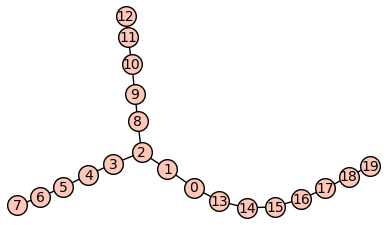
\includegraphics[scale=0.65]{ExtremalTreeExample3(min).png}
			\caption{Extremal tree example minimizing $m(d)$.}\label{Figure-ExtremalTreeExampleMinimizingMultiplicity}
		\end{figure}
	\end{eg}

	\begin{rem}
		Below I conjecture that $d \leq \ceil{n/3}+2$.  I have not yet looked for extremal trees that minimize $m(d)$ when $d \in \{\ceil{n/3}+1, \ceil{n/3}+2\}$.
	\end{rem}
	\newpage
	\begin{conj}
		Let $d$ be the largest distance with max multiplicity in a tree $T$.  
		\begin{enumerate}
			\item If $d \leq C_1\frac{n}{3} + C_2$ and even, then $m(d) \leq (3-a-b)\lceil \frac{r}{3} \rceil \lfloor \frac{r}{3} \rfloor + \lfloor \frac{r}{3} \rfloor^{2a} \lceil \frac{r}{3} \rceil^{2b}$, where $r = n-\tfrac{3}{2}d+2$ and 
			$$(a,b) = \begin{cases}
				(1,0), \text{ if } r \equiv 1 \Mod{3}	\\
				(0,1), \text{ if } r \equiv 2 \Mod{3}	\\
				(0,0), \text{ otherwise. }
			\end{cases}$$
			
			\item If $C_1\frac{n}{3} +C_2< d \leq \lceil \tfrac{n}{3} \rceil + 2$, then $m(d) \leq a\lfloor \frac{r'}{4} \rfloor^2 + (2-a)\lceil \frac{r'}{4} \rceil^2 + 2\lfloor\frac{r'}{4} \rfloor \lceil\frac{r'}{4} \rceil$, where $r' = n-d-1$ and 
			$$a = \begin{cases}
				2, \text{ if } r' \equiv 1 \Mod{4}	\\
				1, \text{ if } r' \equiv 2 \Mod{4}	\\
				0, \text{ otherwise. }
			\end{cases}$$
		\end{enumerate}
	\end{conj}
	
	\begin{rem}
		My experimentation suggests that $C_1 \sim 1$ and $-1 \leq C_2 \leq 1$; however, I have not yet examined these values carefully.
	\end{rem}
	
	
	\begin{rem}
		I believe there are $3$ extremal trees that maximize $m(d)$; one unknown when $d \leq C_1\frac{n}{3} + C_2$ and odd, and the other two are described below.  
	\end{rem}
	
	\begin{prop}[Construction 1]\label{Construction-Small-d-Max-Multiplicity}
		
		Refer to Figure \ref{Figure-ExtremalTreeExamples-a} for an example.  When $d \leq C_1\frac{n}{3}+C_2$ and even, do the following:
		\begin{enumerate}
			\item First we use $3(\frac{d}{2} - 1) + 1$ vertices by making $3$ branch paths with length $\frac{d}{2}-1$ from a root vertex $u$.  
			
			\item Let $v,w,x$ be the vertices at the ends of each branch.  
			
			\item For the remaining $n-3(\frac{d}{2} - 1) - 1$ vertices, append them to $v,w,x$ so that the number of leaf neighbours of $v$, $w$, and $x$ differ from one another by at most $1$.
		\end{enumerate}
	\end{prop} 
	

	\begin{rem}
		Trees with large $m(d)$ when $d  \leq C_1\frac{n}{3} + C_2$ often tend to have a triple branching structure.  The structure of $T$ becomes much more constrained the larger $d$ gets, and I think this is probably because it is most common for $d = 2$.  When $d > 2$, then for $m(2) \leq m(d)$ to hold, \textbf{(1)} the degrees of the vertices of $T$ cannot be too high, and \textbf{(2)} there needs to be enough branching in $T$ to ensure enough distinct length $d$ paths.  Somehow the triple branching pattern in Construction 1 satisfies \textbf{(1)} and \textbf{(2)} while also maximizing $m(d)$; but I doubt that this extremal structure is fragile.  That is, I think even when $d$ is odd and $d  \leq C_1\frac{n}{3} + C_2$, an extremal tree has a similar triple branching structure.
	\end{rem}
	

	\paragraph{Construction 2:} Refer to Figure \ref{Figure-ExtremalTreeExamples-b} for an example.  When $d > C_1\frac{n}{3} + C_2$, do the following:
	\begin{enumerate}
		\item Form a path of length $d-4$ and call its leaves $x$ and $y$.
		
		\item Append two vertices $x_1$ and $x_2$ to $x$ and similarly $y_1$ and $y_2$ to $y$.
		
		\item Append the remaining $n-d-1$ vertices to $x_1$, $y_1$, $x_2$, and $y_2$ so that the number of leaf neighbours on each differ from one another by at most $1$.  If $r' \equiv 2 \Mod{4}$, then ensure that both $x_1$ and $y_1$ are each adjacent to $\ceil{r'/4}$ leaves.
	\end{enumerate}

	\begin{eg}
		Figure \ref{Figure-ExtremalTreeExamples} shows examples from Constructions 1 and 2, which are mentioned above.  In Figure \ref{Figure-ExtremalTreeExamples-a}, $n = 20$, $d = 6$, and $m(6) = 56$.  In Figure \ref{Figure-ExtremalTreeExamples-b}, $n = 24$, $d=\lceil \frac{n}{3} \rceil + 2 = 10$, and $m(d) = 42$.
		
		\begin{figure}[h]
			\centering
			\begin{subfigure}{6.5cm}
				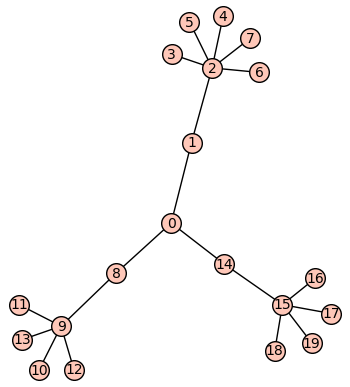
\includegraphics[scale=0.65]{ExtremalTreeExample2.png}
				\caption{Construction 1}\label{Figure-ExtremalTreeExamples-a}
			\end{subfigure}
			\begin{subfigure}{6.5cm}
				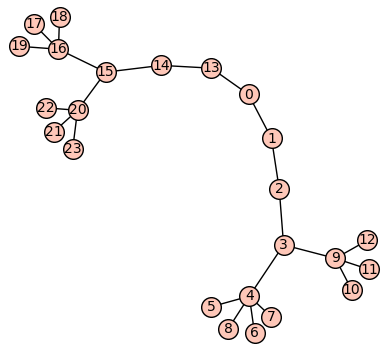
\includegraphics[scale=0.65]{ExtremalTreeExample1.png}
				\caption{Construction 2.}\label{Figure-ExtremalTreeExamples-b}
			\end{subfigure}
			\caption{Extremal tree examples that maximize $m(d)$.}\label{Figure-ExtremalTreeExamples}
		\end{figure}
	\end{eg}

	\begin{conj}
		Let $d$ be the largest distance with max multiplicity.  Then $d \leq \lceil \tfrac{n}{3}\rceil + 2$.
	\end{conj}

	\begin{rem}
		I have not yet found a counter-example to this conjecture.  Please let me know if you find one!  I have searched $n \leq 25$ without finding a CE, but it may well be that $d \leq \ceil{n/3} + C\sqrt{n}$ or something.  If so, then there would probably still be a sensible case division at $d \sim n/3$.
	\end{rem}
	
	
	\iffalse
	\subsection{Constructions}
	
	\begin{prop}
		Let $d$ be the largest distance with max multiplicity.  Then $\min_{T \in \mathcal{T}(n)}m(d) = n-1$.  Let $r = n-3(d/2-1)-1$ and $r' = n-d+1$ and $d$ even.  Then 
		$$\max_{T \in \mathcal{T}(n)}m(d) = \begin{cases}
			\lfloor \tfrac{r}{3} \rfloor(\lfloor \tfrac{r}{3} \rfloor + 2\lceil\tfrac{r}{3} \rceil) & \text{ if } d \leq \tfrac{n}{3}, \text{ and } r \equiv 0,1 \Mod{3}; 	\\
			\lceil \tfrac{r}{3} \rceil(\lceil \tfrac{r}{3} \rceil + 2\lfloor\tfrac{r}{3} \rfloor) & \text{ if } d \leq \tfrac{n}{3}, \text{ and } r \equiv 2 \Mod{3}; 	\\
			
			2\lfloor\tfrac{r'}{4}\rfloor^2 + 2\lfloor\tfrac{r'}{4}\rfloor \lceil\tfrac{r'}{4}\rceil, & \text{ if } d > n/3 \text{ and } r' \equiv 0,1 \Mod{4};	\\
			\lfloor\tfrac{r'}{4}\rfloor^2 + 2\lfloor\tfrac{r'}{4}\rfloor \lceil\tfrac{r'}{4}\rceil + \lceil\tfrac{r'}{4}\rceil^2, & \text{ if } d > n/3 \text{ and } r' \equiv 2 \Mod{4};	\\
			2\lceil\tfrac{r'}{4}\rceil^2 +2\lfloor\tfrac{r'}{4}\rfloor \lceil\tfrac{r'}{4}\rceil, & \text{ if } d > n/3 \text{ and } r' \equiv 3 \Mod{4}.
		\end{cases}$$
	\end{prop}

	\begin{proof}
		When $d \leq \tfrac{n}{3}$, we construct a tree $T$ in two steps.  First we use $3(d/2 + 1) + 1$ vertices by making $3$ branches with length $d-1$ from a root vertex $u$.  Let $v,w,x$ be the vertices at the ends of each branch, respectively.  For the remaining $n-3(d/2 + 1) + 1$ vertices, append them to $v,w,x$ so that the degrees of $v$, $w$, and $x$ differ from one another by at most $1$.  Note that since $d \leq \tfrac{n}{3}$, so $m(2) \leq m(d)$.
	\end{proof}
	\fi
	
	\iffalse
	\section{Crescent Vertices}
	
	Let $v$ be a vertex of a graph $G$.  We say that $v$ is a \emph{crescent vertex} if the multiset of distances from $v$ to every other vertex in $G$ is of the form $\{d_1^{1},d_2^2,\ldots,d_k^{k}\}$ for some $k$.  For example, every vertex in the $4$-cycle $C_4$ is a crescent vertex.  A crescent vertex $v$ has the property that the rest of the vertices can be partitioned into $k$ classes based on the distance from $v$ such that the numbers of vertices in each class is given by a permutation.  We call such a permutation a \emph{crescent permutation}.  For instance, each crescent vertex in $C_4$ induces the crescent permutation $(2,1)$, or $(12)$.  Note that a vertex $v$ is crescent if and only if every other vertex similar to $v$ is crescent, so we are concerned with finding orbits of the given graph that contain crescent vertices.
	
	\begin{question}
		Is $C_4$ the only graph in which every vertex is a crescent vertex?
	\end{question}
	\fi
	
	
	\iffalse
	\section{Hosoya Polynomials}
	
	
	Let $\{d_1^{m_1},d_2^{m_2}, \ldots, d_{k}^{m_k}\}$ be the distance multiset for a graph $G$.  Then the Hosoya polynomial of $G$ is $H_G(x) = \sum_{i=1}^k m_ix^{d_i}$.  Hosoya polynomials appear mainly to just be a reformulation of the distance multiset of $G$, and also $H_G'(1) = \sum_{i=1}^k m_id_i$, which is the sum of all distances in $G$ (often called the Wiener index of $G$).  Note that the Wiener index does not distinguish between which of $d_i$ or $m_i$ is a distinct distance or multiplicity.  Thus for example the Hosoya polynomial for a graph $K$ with $H_K(x) = \sum_{i = 1}^k d_ix^{m_i}$ satisfies $H_K'(1) = H_G'(1)$.  In general, if two distinct graphs $G$ and $K$ have the same Wiener index, does this impose any constraints on the multiplicities of particular distances of $G$ and $K$?  More constraints on $G$ and $K$ are probably needed.  I explore some below.
	
	Suppose $G$ and $K$ have the same order and distances $d_1, d_2, \ldots, d_k$.  Note that if $G$ and $K$ are unlabelled graphs (as opposed to edge-labelled graphs, say), then these distances must be $1, 2, \ldots, k$, where $k = \diam(G) = \diam(K)$.  Represent these distances as a vector $x$, and similarly the multiplicities of $G$, $y = (m_1, m_2, \ldots, m_k)$ and those of $K$, $z = (m_1', m_2', \ldots, m_k')$.  Then if $w(G)$ is the Wiener index of $G$, $xy = xz = w(G)$.  
	
	We can make a matrix $A$ here where $Ax = w \mathbf{1}$.  Sticking with the unlabelled graph case, if the rows of $A$ are multiplicity lists for the distances $1, 2, \ldots, k$ corresponding to graphs with Wiener index $w(G)$, then $\tfrac{Ax}{w(G)} = \mathbf{1}$.  I believe $w(G)$ tells us something about the multiplicity distribution.  In particular, if $w(G)$ is large, then the multiplicities of the large distances should be higher, and if $w(G)$ is small, then the large distance should have smaller multiplicities.  Thus if $H_G'(1) = H_K'(1)$, then we should expect the average difference in multiplicities between $G$ and $K$ to be small; that is, $\tfrac{1}{k}\sum_{i=1}^k |m_i - m_i'|$ should be relatively small.  
	
	
	Here's an attempt:  Let $G$ be a graph with distances $1, 2, \ldots, k$ and respective multiplicities $m_1, m_2, \ldots, m_k$.  Let $y_i$ be the vector $(m_1, m_2, \ldots, m_{i-1}, i, m_{i+1}, \ldots, m_k)$, that is, with $m_i$ swapped for its distance $i$.  Then let $A$ be the matrix with $y_1, y_2, \ldots, y_k$ as row vectors.  Then $Ax = w \mathbf{1}$.  If 
	
	If $x = (1, 2, \ldots, k)$, then I think the average difference $m_i - m_i'$ has to be close to $0$, since otherwise
	
	
	There are 3 main points:
	
	Another construction that tries to minimize mult(d) and mult(2) given that d is the largest distance with maximum multiplicity.  The theme I want to develop here is that if mult(d) = max mult, then mult(2) is very close to mult(d) and minimizing mult(d) can often be achieved by minimizing mult(2) (fewer large degree vertices and smaller max degree).
	Hosoya polynomials seem to provide a way to compare related crescent configuration graph G and H whose multiplicities are a permutation of the distances 1,2, ..., n-1.  Here "related" means (1) G and H have the same Wiener index (sum of all distances), and (2) H has the same distances as G except that some of its distinct distance
	
	
	
	
	A Hosoya polynomial is a degree $k$ polynomial $H(x) = c_0 + c_1x + \cdots + c_kx^k$ in which $c_0 = 0$, and $c_i$ is a positive integer for all $i \in [k]$. This polynomial has the property that its first derivative $H'(x) = \sum_{i=1}^{k}ic_ix^{i-1}$ satisfies $H'(1) = \sum_{i=1}^{k} ic_i$.  Hosoya polynomials were introduced by [so and so] in which $H(x)$ describes the distance multiset of a class of graphs whereby $c_i$ is the multiplicity of distance $i$.  In this graph context where $H(x) = H_\mathcal{G}(x)$ is the Hosoya polynomial for a graph class $\mathcal{G}$, the value $H'(1)$ is the sum of all distances between the vertices in a graph in $\mathcal{G}$; this quantity is called the Wiener index of a graph.  In this section, we make the case that Hosoya polynomials do more than just efficiently represent the distance multiset of a graph, but actually describe a correspondence between graphs with the same Wiener index.
	
	\begin{obs}
		Let $\mathcal{G}$ be a class of edge-weighted graphs of order $n$ with distinct distances $1, 2, \ldots, n-1$ and corresponding Hosoya polynomial $H_\mathcal{G}(x) = \sum_{i=1}^{n-1} \sigma(i)x^{i}$ for some permutation $\sigma$ on $\mathcal{S}_{n-1}$.  Then 
		
		\begin{enumerate}
			\item Each graph in $\mathcal{G}$ is a crescent configuration graph
			\item For each product of disjoint cycles $\tau$ of $\sigma$, the Hosoya polynomial $H_\mathcal{K}(x) = \sum_{i=1}^{n-1} \tau^{-2}\sigma(i)x^{i}$ satisfies $H_\mathcal{K}'(1) = H_\mathcal{G}'(1)$.  
			
			\begin{itemize}
				\item That is, $\tau$ corresponds to a Hosoya polynomial that corresponds to a (\textbf{possibly empty}) class of crescent configuration graphs $\mathcal{K}$ that have the same Wiener index as those in $\mathcal{G}$.  
				\item Essentially, this observation leverages the idea that the Wiener index calculation does not distinguish between multiplicities and distances.  
				\item The permutation structure comes from the fact that we are working with the crescent pattern, which can define a permutation between distinct distances and multiplicities.
				
				\item Note that if $\sigma$ has $b$ disjoint cycles, then there are $2^b$ distinct Hosoya polynomials, each corresponding to a (possibly nonempty) class of crescent configuration graphs related to those in $G$.  Each polynomial can be imagined as a vertex on the hypercube $Q_b$ (each has the same Wiener index and are based on $\sigma$).
				
				\item Note that the polynomial $\sum_{i=1}^{n-1} \sigma^{-1}(i)x^i$ corresponds to the class of crescent configuration graphs with distances and multiplicities equal to the multiplicities and distances, respectively, of those in $\mathcal{G}$.  It might be interesting to compare graphs that manage to have the same Wiener index with their distances and multiplicities swapped.  It's weird to think of distinct distances and multiplicities as interchangeable in this way!
			\end{itemize}
		
			\item Note that $H_G(x) - H_K(x) = \sum_{i=1}^{k}(c_i-r_i)x^{i} = \sum_{i=1}^k c_ix^i - \sum_{j=1}^k$
		\end{enumerate}
		
	\end{obs}

	Note that 
	\begin{align*}
		H_G'(x) - H_K'(x) &= \sum_{i=1}^{k}i(\sigma(i)-\tau^{-2}\sigma(i))x^{i-1}	\\
		&= \sum_{i \in \tau} i(\tau(i)-\tau^{-1}(i))x^{i-1} + \sum_{\substack{i \notin \tau \\ i \in [n-1]}} i(\sigma(i)-\sigma(i))x^{i-1}	\\
		&= \sum_{i \in \tau} i(\tau(i)-\tau^{-1}(i))x^{i-1} + 0	\\
	\end{align*}
	
	So if $\tau = (abc)$, say, then this difference is $a(b-c)x^{a-1} + b(c-a)x^{b-1} + c(a-b)x^{c-1}$.  In particular, when $x=1$, we have $a(b-c) + b(c-a) + c(a-b) = 0$.

	\begin{proof}
		We have that
		\begin{align*}
			H_G'(1) &= H_K'(1)	\\
			\Leftrightarrow \sum_{i=1}^{k} ic_i &= \sum_{i=1}^{k} ir_i	\\
			\Leftrightarrow \sum_{i=1}^{k} i(c_i-r_i) &= 0
		\end{align*}
	
		Note that $H_G'(x) - H_K'(x) = \sum_{i=1}^{k}i(c_i-r_i)x^{i-1}$.
		
		Note that $H_G(x) - H_K(x) = \sum_{i=1}^{k}(c_i-r_i)x^{i}$
	\end{proof}
	\fi
	
	\section{Construction with Large Gap Between Max Multiplicity and $\mathbf{\mult(2)}$}
	
	Let $G$ be a tree of order $n$ and max degree $\Delta$.  Let $d$ be an even distance in $\{2,4,\ldots, n-1\}$ with maximum multiplicity in $G$.  Given $\Delta$ and $d$, the following construction attempts to maximize $\mult(d)$ while minimizing $\mult(2)$.  The idea is to create a tree $G$ where all vertices either have degree $1$ or $\Delta$ and each path of length $d$ has end-vertices with degree $1$ in $G$.  Note that these conditions determine a value of $n = n(d,\Delta)$.  Recall from Proposition \ref{Proposition-Minimizing-m(d)-to(n-1)} and corresponding Figure \ref{Figure-ExtremalTreeExampleMinimizingMultiplicity} that we can minimize $\mult(d)$ at $\mult(2) = n-1$.  Similarly, in the construction from Proposition \ref{Construction-Small-d-Max-Multiplicity}, we had $\mult(2) = \mathcal{O}((\tfrac{n}{3}-\tfrac{3d}{2})^2)$ with $\mult(d) = \mathcal{O}(n^2)$, which are asymptotically equivalent when $d$ is not a function of $n$.  The purpose of the following construction is to show that $\mult(d)$ need not be close to $\mult(2)$; in fact, we will see that it is possible for $\mult(d) = \mathcal{O}(n^2)$ while $\mult(2) = \mathcal{O}(n\Delta)$.
	
	\paragraph{Construction.} Let $d$ and $\Delta$ be positive integers such that $d$ is even.  We construct a graph $G(d,\Delta)$ as follows:
	\begin{enumerate}
		\item Let $r$ be a vertex with neighbours $v_{1},v_{2}, \ldots, v_{\Delta}$.
		
		\item For each $j \in [\Delta]$, identify $v_{j}$ with the root of a $(\Delta-1)$-ary tree with depth $\tfrac{d}{2}-1$.
	\end{enumerate}
	
	\begin{eg}
		Let $(d,\Delta) = (6,4)$.  Then the following tree of order $53$ results from the above construction:
		\begin{figure}[h]
			\begin{center}
				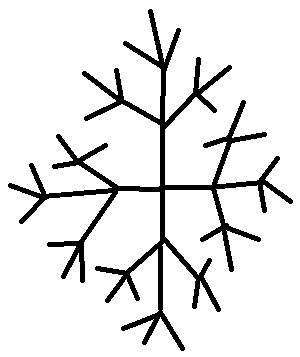
\includegraphics[scale = 0.5]{Delta-ary-tree-example.png}
			\end{center}
			\caption{Example of a tree satisfying $(n,d,\Delta) = (53,6,4)$ where $\mult(2) = 102$ and $\mult(d) = 486$.}
		\end{figure}
	\end{eg}
	
	Let $n_1$ and $n_\Delta$ denote the numbers of vertices with degrees $1$ and $\Delta$, respectively.  We can express both $n_1$ and $n_\Delta$ as functions of $\Delta$ and $d$, and since $n = n_1 + n_\Delta$, we can do the same for $n$.  Note that the eccentricity of the root vertex is $\tfrac{d}{2}$.  We can count the number of vertices by summing the number of vertices at distance $i \in \{0,1, \ldots, \tfrac{d}{2}\}$ from the root.  We have:
	\begin{align*}
		n &= 1 + \Delta + \Delta(\Delta-1) + \cdots + \Delta(\Delta-1)^{\tfrac{d}{2}-1}	\\
		&= 1 + \Delta\sum_{i=0}^{\tfrac{d}{2}-1}(\Delta - 1)^i.
	\end{align*}

	Note that from this we have $n_1 = \Delta(\Delta-1)^{\tfrac{d}{2}-1} = \mathcal{O}(\Delta^{\tfrac{d}{2}})$, and since $n_1 > n_\Delta$, we have $n = n_1 + n_\Delta = \mathcal{O}(\Delta^{\tfrac{d}{2}})$ as well.  The paths with length $d$ always have end-vertices being leaves of $G$ in the $\Delta$ distinct branches from the root of $G$.  There are $(\Delta-1)^{\tfrac{d}{2}-1}$ leaves in each of these $\Delta$ branches, so $\mult(d) = {\Delta \choose 2}(\Delta-1)^{d-2} = \mathcal{O}(\Delta^d)$.  For $\mult(2)$, we sum the ${\Delta \choose 2}$ distinct paths of length $2$ at each of the $1 + \Delta\sum_{i=0}^{\tfrac{d}{2}-2}(\Delta - 1)^i$ non-leaf vertices.  So, $\mult(2) = {\Delta \choose 2}(1 + \Delta\sum_{i=0}^{\tfrac{d}{2}-2}(\Delta - 1)^i) = \mathcal{O}(\Delta^{\tfrac{d}{2}+1})$, and putting all these in terms of $n$, we have $\mult(d) = \mathcal{O}(n^2)$ and $\mult(2) = \mathcal{O}(n\Delta)$, which is quite a large distance.  Thus it is possible to construct trees where the largest distance with maximum multiplicity has multiplicity much larger than the multiplicity of $2$.
	
	The following conjecture reflects the intuition that if distances $2$ and $d = \diam(G)$ have similar multiplicities, then there are few vertices with high degree and little branching.
	
	\begin{conj}
		Let $G$ be a tree with even diameter $d$ where $d$ is the largest distance with maximum multiplicity.  If $\mult(2) \sim \mult(d)$, then there are at most $3$ vertex disjoint paths between the centre and periphery of $G$.
	\end{conj}
	
	\iffalse
	\section{Understanding Distance Multiset Structure Given Graph Symmetry}
	
	The underlying idea here is that we may want to consider ways of partitioning the vertices into classes, whereby we know a lot about the distances between these classes.  The main hypothesis I am proposing is that if we can account for all but $Cn$ of the distances, then we can say a lot about the distance multiset structure of the graph.  For example, we could ignore $C$ pesky vertices that break symmetry, and then use the unbroken symmetry to come up with a nice vertex partition.
	
	What follows is a more detailed example approach.  Observe that if a graph $G$ has a high amount of symmetry, we can sometimes partition $V(G)$ into classes $V_1, V_2, \ldots, V_k$ where the \textit{external} distances between distinct classes $V_i$ and $V_j$ are known, or are even all equal to some small distance multiset $D$.  For instance, the vertices of the graph on $6$ vertices that is a union of a $C_6$ $(v_1v_2v_3v_4v_5v_6v_1)$ and the edge $v_2v_5$ can be partitioned into $\{v_1,v_4\}$, $\{v_2,v_5\}$, and $\{v_3,v_6\}$ whereby the distances between each class is given by the distance multiset $D = \{1^2,2^2\}$.  We have that all but three of the distances are external, which are given by $3$ copies of $D$, $\{1^6,2^6\}$.  The internal distances are $\{1^1,3^2\}$.  In this case, since the external distances are the majority and easily characterized, we can say a lot about the distance multiset of the graph based on external distances only.  For example, the max multiplicity is at least $6$, only distances $1$ or $2$ can have max multiplicity, and since each class has at most ${2 \choose 2} = 1$ edges, the diameter of the graph has to be at most $1 + \max(D) = 3$.
	
	A big picture question is: which graphs have distance multisets that have easy to characterize distance multisets if we ignore distances between only a small number of pesky vertices.  
	
	\paragraph{Trees.} For instance, if we have a tree of order $n$ and we know there are $k$ vertices $v_1, v_2, \ldots, v_k$ such that $\deg(v_i) \geq \ell+1$ and they are all distance $x$ apart from one another, then $\mult(x) \geq {k \choose 2} \ell^2$.  The more general observation is that even if these vertices aren't equidistant, there are at most ${k \choose 2}$ distinct distances that receive multiplicity in multiples of $\ell^2$.
	
	Suppose $n = (k+1)\ell + C$ where there are $k$ vertices with degree at least $\ell + 1$.  Then ${k \choose 2}\ell^2$ of the distances occur between these $k$ stars, and $(k+1)\ell C + {C \choose 2}$ distances involve the $C$ vertices outside the stars.  If $(k+1)\ell = \mathcal{O}(n)$ and $C$ is a constant, then the number of distances involving vertices outside the stars is $\mathcal{O}(n)$.  This means that as $n$ gets big, the distance multiset of the tree is mostly described by the distances between stars, which contribute multiplicity in multiples of $\ell^2$.
	
	For example, suppose $k \sim \tfrac{n-10}{10}$, $\ell = 10$, and $C = 10$.  Then there are around $(n-10)10 + 50 = 10n - 50$ distances involving the $10$ non-star vertices.  There are around $\tfrac{(n-10)^2}{2}$ distances between stars, and they contribute multiplicity in multiples of $\ell^2 = 100$.  I think this means we should expect jumps in multiplicity on the order of something like $\ell^2$.  Put another way, $\ell$ might be relate to the slope of the multiplicity distribution.
	\fi
	
	\newpage
	
	\section{Distance Multisets of Specific Graphs}
	
	\subsection{Paths, Cycles, and Grid Graphs}
	
	\begin{obs}
		Paths of order $n$ have distance multiset $\{1^{n-1},2^{n-2}, \ldots, (n-1)^1\}$.
	\end{obs}
	
	\begin{obs}
		Odd cycles of order $n$ have distance multiset $\{1^n, 2^n, \ldots, \floor{\tfrac{n}{2}}^n\}$.  Even cycles of order $n$ have distance multiset $\{1^n, 2^n, \ldots, (\tfrac{n}{2}-1)^n, (\tfrac{n}{2})^{\tfrac{n}{2}}\}$.
	\end{obs}
	
	\begin{prop}
		Let $a$ and $b$ be positive integers such that $a \geq b$.  Then the multiplicity of each distance $x$ in the $a$ by $b$ grid graph is given by
		\begin{align*}
			\mult(x) = 
			\begin{cases}
				(2bx-x^2)a + 2{x+1 \choose 3} - bx^2, &\text{if } x \in [1,b-1];	\\
				b^2(a-x) + 2{b+1 \choose 3}, &\text{if }x \in [b,a-1];	\\
				2{b+1 - (x-a) \choose 3}, &\text{if }x \in [a,a-1+b-1].
			\end{cases}
		\end{align*}
	\end{prop}
	
	\begin{proof}
	
	%	  Note that the distance of $G_{a,b}$ are the internal distances of $G_{a,b-1}$ and $P_a$ along with the external distances between a $G_{a,b-1}$ and $P_a$.
		
	%	Let $P_a = (v_1,v_2,\ldots, v_{a})$.  Note for each $i \in [0,\floor{a/2}]$ that $v_i$ and $v_{a-i}$ have the same distances with $G_{a,b-1}$.  We can partition $V(G_{a,b-1})$ into $a$ $P_{b-1}$s, call them $P(1), P(2), \ldots, P(a)$.  Suppose $v_i$ is adjacent to an end-vertex in $P(i)$.  For a given $i \in [0,\tfrac{a}{2}]$, for all $j \in [i,a]$, then the distances between $v_i$ and $P(j)$ are $\{1, 2, \ldots, b-1\} + j-i$; similarly, for all $j \in [1,i-1]$, the distances between $v_i$ and $P(j)$ are $\{1, 2, \ldots, b-1\} + i-j$.
		
	%	So, the distances $\{1, 2, \ldots, b-1\}$ occur $a$ times, $\{1, 2, \ldots, b-1\}+1$ occur $a-1$ times, and in general $\{1, 2, \ldots, b-1\} + i$ occur $a-i$ times.  Similarly, the distances $\{1, 2, \ldots, b-1\} + a-i$ occurs $i$ times.  So, when $i = 0$, distance $d$ occurs $a$ times...[need to finish].
		
	%	Nevermind the above setup.
		
	%	We want to calculate the distances between each $v_1, v_2, \ldots, v_a$ and the vertices in $P(1), P(2), \ldots, P(a)$.  There are $a^2$ such $(v_i,P(j))$ pairs where $i, j \in [a]$.  Note that the distances between $v_i$ and $v_j$ are $\{1, 2, \ldots, b-1\}+|i-j|$.  Since $v_1, v_2, \ldots, v_a$ form a path, it is straightforward to see that when $d \in \{1, 2, \ldots, a-1\}$, there are $2(a-d)$ pairs $(i,j)$ such that $|i-j| = d$.  When $d = 0$, then $i = j$ and there are $a$ such pairs.  So, for $d \in [a-1]$, there are $2(a-d)$ occurrences of the distances $\{1, 2, \ldots, b-1\} + d$ between $P_a$ and $G_{a,b-1}$ and $a$ occurrences of $\{1, 2, \ldots, b-1\}$.  Thus we have for the distances between $1$ and $b-1$: $1^a$, $2^{a+2(a-1)}$, $3^{a+2(a-1)+2(a-2)}$, $\ldots$, $(b-1)^{a+\sum_{d=1}^{b-2}2(a-d)}$.  In general, we have external distance $x \in [b-1]$ occurs with multiplicity ${a + \sum_{d=1}^{x-1}2(a-d)}$.  Then the multiplicities of the rest of the external distances $b$ through $a-1 + b-1$ are calculated differently: $b^{\sum_{d=1}^{b-1} 2(a-d)}$, $(b+1)^{\sum_{d=2}^{b}2(a-d)}$, and in general, for all $\ell \in \{0, 1, \ldots, a-2\}$, we have $(b+\ell)^{\sum_{d=\ell+1}^{\ell + b-1} 2(a-d)}$.
		
	%	We can simplify these sums.  Note that $\sum_{d=1}^{x-1}2(a-d) = 2a(x-1) - x(x-1) = (x-1)(2a-x)$, and $\sum_{d=\ell+1}^{\ell + b-1} 2(a-d) = 2a(b-1) - 2\sum_{d=\ell+1}^{\ell+b-1}d = 2a(b-1) - 2(b-1)(\ell+1) - 2{b-1 \choose 2} = 2a(b-1)-2(b-1)(\ell+1) - (b-1)(b-2) = (b-1)(2a-2(\ell+1)-(b-2))$.  Therefore, if $x = b + \ell$, then substituting $x-b$ for $\ell$ we get that distance $x \in \{b, b+1, \ldots, b+a-2\}$ has multiplicity $(b-1)(2a-2(x-b+1)-(b-2))$.  Thus the external distances between $G_{a,{b-1}}$ and $P_a$ are 
	%	$$\{x^{a+(x-1)(2a-x)}: x \in \{1, 2, \ldots b-1\}\} \cup \{x^{(b-1)(2a-2(x-b+1)-(b-2))}: x \in \{b, b+1, \ldots, b-1 + a-1\}\}.$$
		
	%	We still need to determine the distances of $G_{a,b-1}$ though.  We can start with $G_{a,1}$ and since we know how many distances are added, we can count recursively.  $G_{a,1}$ has distances $\{1^{a-1}, 2^{a-2}, \ldots, (a-1)^1\}$, then by above, $G_{a,2}$ has distances $\{1^{a-1}, 2^{a-2}, \ldots, (a-1)^1\}$ from $G_{a,1}$ and $P_a$ and also
	%	$$\{1^{a}\} \cup \{x^{2a-2(x-1)}: x \in \{2, 3, \ldots, a\}\}.$$
		
	%	Altogether $G_{a,2}$ has distance multiset $\{1^{3a-2}\} \cup \{x^{2a-2(x-1) + 2(a-x)}: x \in \{2, 3, \ldots, a-1\}\} \cup \{a^{2}\}$.  \textbf{More simplified:} $\{1^{3a-2}\} \cup \{x^{4(a-x)+2}: x \in \{2, 3, \ldots, a-1\}\} \cup \{a^{2}\}$.
		
	%	To find the closed form expression, we will need to find the distances in $G_{a,3}$.  Note the distances are
		
	%	$\{1^{3a-2}\} \cup \{x^{4(a-x)+2}: x \in \{2, 3, \ldots, a-1\}\} \cup \{a^{2}\}$ unioned with $\{1^{a-1}, 2^{a-2}, \ldots, (a-1)^1\}$ and also
		
	%	$$\{x^{a+(x-1)(2a-x)}: x \in \{1, 2\}\} \cup \{x^{(2)(2a-2(x-2)-1)}: x \in \{3, 4, \ldots, a+1\}\}.$$
		
	%	So the distance multiset of $G_{a,3}$ is
		
	%	$$\{1^{3a-2+(a-1)+a}\} \cup \{2^{4(a-2)+2 + (a-2) +a + (2a-2)}\} \cup \{x^{4(a-x)+2 + (a-x) + 2(2a-2(x-2)-1)}: x \in \{3, 4, \ldots, a-1\}\}$$
		
	%	unioned with $\{a^{2 + 2(2a-2(a-2)-1)}\} \cup \{(a+1)^{2(2a-2(a-1)-1)}\}$.
		
	%	\textbf{More simply:}
		
	%	$$\{1^{5a-3}, 2^{8a-10}\} \cup \{x^{9(a-x)+8}: x \in \{3, 4, \ldots, a-1\}\} \cup \{a^{8}, (a+1)^{2}\}.$$
		
	%	Gotta figure out $G_{a,4}$... Okay, it is the union of:
	%	\begin{enumerate}
	%		\item $\{1^{5a-3}, 2^{8a-10}\} \cup \{x^{9(a-x)+8}: x \in \{3, 4, \ldots, a-1\}\} \cup \{a^{8}, (a+1)^{2}\}.$
	%		\item $\{1^{a-1}, 2^{a-2}, \ldots, (a-1)^1\}$,
	%		\item $\{x^{a+(x-1)(2a-x)}: x \in \{1, 2, 3\}\} \cup \{x^{3(2a-2(x-3)-2)}: x \in \{4, 5, \ldots, a+2\}\}.$
	%	\end{enumerate}
	
	%Altogether, we have that the distances in $G_{a,4}$ are:
	
	%$\{1^{5a-3+a-1+a}, 2^{8a-10 + a-2 + a+2a-2}, 3^{9(a-3)+8 + a-3 + a+2(2a-3)}\}$ along with $\{x^{9(a-x)+8 + a-x + 3(2a-2(x-3)-2)}: x \in \{4, 5, \ldots, a-1\}\}$, %along with $\{a^{8 + 3(2a-2(a-3)-2)}, (a+1)^{2 + 3(2a-2(a-2)-2)}, (a+2)^{3(2a-2(a-1)-2)}\}$.
	
	%More simply, we have:
	
	%$$\{1^{7a-4}, 2^{12a-14}, 3^{15a -28}\} \cup \{x^{16(a-x) + 20}: x \in \{4, 5, \ldots, a-1\}\} \cup \{a^{20}, (a+1)^{8}, (a+2)^{2}\}$$
	
	%Dang okay, I made a mistake in the external distance calculation.  The fix is below.  Fortunately, it's much simpler!
	
	Let $G_{a,b}$ be the grid graph with dimensions $a$ and $b$.  We first find a recurrence relation by calculating the distances between two vertex disjoint induced subgraphs of $G_{a,b}$: $G_{a,b-1}$ and a path of length $a-1$, which we call $P_a$.  We call such distances ``external distances", and the distances between vertices within $G_{a,b-1}$ and within $P_{a}$ are called ``internal distances".  Throughout this proof, for a distance $x \in [1, a-1+b-1]$, we often distinguish between the internal and external multiplicities of $x$.  It is straightforward to see that the distances of $G_{a,b}$ are the union of external and internal distances between $G_{a,b-1}$ and $P_a$.  Once we know how to find these external distances, we will use this relation in a proof by induction to obtain the closed form expression for the distance multiset of $G_{a,b}$.  
	
	Let $v_1, v_2, \ldots, v_a$ be the vertices of $P_a$, and let $P(j)$ denote the path subgraph of $G_{a,b}$ with length $b-1$ such that $v_j$ is one of its end-vertices.  Note that $\{P(j):j \in [a]\}$ partitions $V(G_{a,b})$ and there are $a^2$ ways to pair these paths with the vertices of $P_a$.  
	
	For a distance $x \in [1,b-1]$, there are $2(a-d)$ ordered pairs $(i,j) \in [a]^2$ such that $|i-j| = d$, and each of these corresponds to an external distance $x$.  The external multiplicity of $x$ is given by $a + \sum_{d=1}^{x-1}2(a-d)$, where the upper limit of $x-1$ ensures that we are ignoring internal distances within $P_a$.  The $a$ term comes from the $a$ pairs $(i,j)$ such that $|i-j| = 0$.  
	
	When $x \in [b,a-1]$, the external multiplicity is given by $\sum_{d=x-(b-1)}^{x-1}2(a-d)$.  In this case, we have to ignore smaller differences (\textit{i.e.}, those less than $x-(b-1)$) in $P_a$ since $x \geq b-1$.  When $x \in [a,a-1+b-1]$, the external multiplicity of $x$ is $\sum_{d=x-(b-1)}^{a-1}2(a-d)$. [\textbf{Probably should include pictures to illustrate these three cases}]  We can simplify these expressions as follows:
	

\paragraph{Case 1:}When $x \in [1,b-1]$, 
			$$a + \sum_{d=1}^{x-1}2(a-d) = a + 2a(x-1) - x(x-1) 
			= a+(x-1)(2a-x).$$
\paragraph{Case 2:}	When $x \in [b,a-1]$,
		$$\sum_{d=x-(b-1)}^{x-1}2(a-d) = 2a(b-1) - 2(b-1)(x-(b-1)) - (b-1)(b-2)
		=(b-1)(2a -2x + b).$$
		%\begin{align*}
		%	\sum_{d=x-(b-1)}^{x-1}2(a-d) &= 2a(b-1) - 2(b-1)(x-(b-1)) - (b-1)(b-2)	\\
			%&= (b-1)(2a - 2(x-(b-1)) - (b-2))	\\
			%&= (b-1)(2a - 2x + 2b - 2 - b + 2)	\\
		%	&= (b-1)(2a -2x + b)
		%\end{align*}
	
\paragraph{Case 3:} When $x \in [a,a-1 + b-1]$,
		\begin{align*}
			\sum_{d=x-(b-1)}^{a-1}2(a-d) &= 2a(a-x+b-1) - 2(a-x+b-1)(x-(b-1)) - (a-x+b-1)(a-x+b-2)	\\
			&= (a-x+b-1)(2a-2(x-b+1) - a + x - b + 2)	\\
			%&= (a+b-1-x)(2a-2x + 2b - 2 - a + x - b + 2)	\\
			&= (a+b-x-1)(a+b-x)
		\end{align*}

	Altogether, the external distances between $G_{a,b-1}$ and $P_a$ are:
	\begin{align*}
		\mult(x)_{Ext} =
		\begin{cases}
			a+(x-1)(2a-x), &\text{if } x \in [1,b-1];	\\
			(b-1)(2a-2x+b), &\text{if } x \in [b,a-1];	\\
			2{a+b-x \choose 2}, &\text{if } x \in [a,a-1+b-1].
		\end{cases}
	\end{align*}
	
	
	
	\iffalse
	In $G_{a,1}$, we have $\{x^{a-x}: x \in [a-1]\}$.  In $G_{a,2}$, the internal distances are $\{x^{2(a-x)}: x \in [a-1]\}$ and the external distances are:
	
	$$\{1^{a}\} \cup \{x^{2a-2x+2}: x \in [2,a-1]\} \cup \{a^{2}\}.$$
	
	Altogether, the distances of $G_{a,2}$ are:
	
	$$\{1^{3a-2}\} \cup \{x^{4(a-x)+2}: x \in [2,a-1]\} \cup \{a^2\}.$$
	
	For $G_{a,3}$, the internal distances are $\{1^{3a-2}\} \cup \{x^{4(a-x)+2}: x \in [2,a-1]\} \cup \{a^2\}$ and $\{x^{a-x}: x \in [a-1]\}$, which together is:
	$$\{1^{4a-3}\} \cup \{x^{5(a-x)+2}: x \in [2,a-1]\} \cup \{a^2\},$$
	and the external distances are:
	$$ \{1^{a}, 2^{3a-2}\} \cup \{x^{2(2a-2x+3)}: x \in [3,a-1]\} \cup \{a^{6}, (a+1)^2\}.$$
	
	Then altogether we have that the distances of $G_{a,3}$ are:
	
	$$\{1^{5a-3}, 2^{8a-10}\} \cup \{x^{9(a-x)+8}: x \in [3,a-1]\} \cup \{a^8,(a+1)^2\}.$$
	
	
	Now for $G_{a,4}$.
	
	The internal distances are 
	$$\{1^{6a-4}, 2^{9a-12}\} \cup \{x^{10(a-x)+8}: x \in [3,a-1]\} \cup \{a^8,(a+1)^2\}.$$
	
	The external distances:
	
	$$ \{1^{a}, 2^{3a-2}, 3^{5a-6}\} \cup \{x^{3(2a-2x+4)}: x \in [4,a-1]\} \cup \{a^{12},(a+1)^{6},(a+2)^{2}\}.$$
	
	Altogether, the distances for $G_{a,4}$ are:
	
	$$ \{1^{7a-4}, 2^{12a-14}, 3^{15a-28}\} \cup \{x^{16(a-x)+20}: x \in \{4,a-1\}\} \cup \{a^{20}, (a+1)^{8}, (a+2)^2\}.$$
	
	I think I need one more:
	
	The internal distances of $G_{a,5}$ are:
	
	$$ \{1^{8a-5}, 2^{13a-16}, 3^{16a-31}\} \cup \{x^{17(a-x)+20}: x \in \{4,a-1\}\} \cup \{a^{20}, (a+1)^{8}, (a+2)^2\}.$$
	
	The external distances are:
	
	$$ \{1^{a}, 2^{3a-2}, 3^{5a-6}, 4^{7a-12}\} \cup \{x^{4(2a-2x+5)}: x \in [5,a-1]\} \cup \{a^{20}, (a+1)^{12}, (a+2)^{6}, (a+3)^2\}.$$
	
	Altogether the distances of $G_{a,5}$ are:
	
	$$\{1^{9a-5}, 2^{16a-18}, 3^{21a - 37}, 4^{24a - 60}\} \cup \{x^{25(a-x)+40}: x \in [5,a-1]\} \cup \{a^{40}, (a+1)^{20}, (a+2)^8, (a+3)^2\}.$$
	\fi
	
	Now we use this to find the distances in $G_{a,b}$.  Below are the distance multisets of $G_{a,2}$, $G_{a,3}$, $G_{a,4}$, and $G_{a,5}$.
	\begin{align*}
		G_{a,2} &\Rightarrow \{1^{3a-2}\} \cup \{x^{4(a-x)+2}: x \in [2,a-1]\} \cup \{a^2\}.	\\
		G_{a,3} &\Rightarrow \{1^{5a-3}, 2^{8a-10}\} \cup \{x^{9(a-x)+8}: x \in [3,a-1]\} \cup \{a^8,(a+1)^2\}.	\\
		G_{a,4} &\Rightarrow \{1^{7a-4}, 2^{12a-14}, 3^{15a-28}\} \cup \{x^{16(a-x)+20}: x \in \{4,a-1\}\} \cup \{a^{20}, (a+1)^{8}, (a+2)^2\}.	\\
		G_{a,5} &\Rightarrow \{1^{9a-5}, 2^{16a-18}, 3^{21a - 37}, 4^{24a - 60}\} \cup \{x^{25(a-x)+40}: x \in [5,a-1]\} \cup \{a^{40}, (a+1)^{20}, (a+2)^8, (a+3)^2\}.
	\end{align*}
	
	
	%I think I see it.
	
	We claim that the distance multiset of $G_{a,b}$ is given by
	\begin{align*}
		\mult(x) = 
		\begin{cases}
			(2bx-x^2)a + 2{x+1 \choose 3} - bx^2, &\text{if } x \in [1,b-1];	\\
			b^2(a-x) + 2{b+1 \choose 3}, &\text{if }x \in [b,a-1];	\\
			2{b+1 - (x-a) \choose 3}, &\text{if }x \in [a,a-1+b-1].
		\end{cases}
	\end{align*}
	
	
	%We have $\{x^{2{b+1 - (x-a) \choose 3}}: x \in [a,a-1+b-1]\}$.  Also, $\{x^{b^2(a-x) + 2{b+1 \choose 3}}: x \in [b,a-1]\}$.  Additionally, $\{x^{(2bx-x^2)a - \tfrac{x(x+1)(2x+1)}{3} - (b-1-x)x^2}: x \in [1,b-1]\}$.
	
	%For the latter multiplicities, we can simplify the expression further:
	%\begin{align*}
	%	(2bx-x^2)a - \tfrac{x(x+1)(2x+1)}{3} - (b-1-x)x^2 &= (2bx-x^2)a + \frac{(x-1)x(x+1)}{3} - bx^2	\\
	%	&= (2bx-x^2)a + 2{x+1 \choose 3} - bx^2
	%\end{align*}
	
	This is our inductive hypothesis.  Note that the base cases are satisfied by our claimed solution.  We now begin the inductive step of the proof.  By the inductive hypothesis, the cumulative internal distance multiplicities of $G_{a,b-1}$ and $P_a$ for distance $x$ are
		\begin{align*}
			\mult(x)_{Int} = 
			\begin{cases}
				(2(b-1)x-x^2)a + 2{x+1 \choose 3} - (b-1)x^2 + (a-x), &\text{if } x \in [1,b-2];	\\
				(b-1)^2(a-x) + 2{b \choose 3} + (a-x), &\text{if }x \in [b-1,a-1];	\\
				2{b - (x-a) \choose 3}, &\text{if }x \in [a,a-1+b-2].
			\end{cases}
		\end{align*}
	Note that we simply add $(a-x)$ (the internal multiplicity of $x$ within $P_a$) to the internal multiplicities of $G_{a,b-1}$ when $x \in [1,a-1]$.
	We showed earlier that the external distance multiplicities between $G_{a,b-1}$ and $P_a$ are
	\begin{align*}
		\mult(x)_{Ext} =
		\begin{cases}
			a+(x-1)(2a-x), &\text{if } x \in [1,b-1];	\\
			(b-1)(2a-2x+b), &\text{if } x \in [b,a-1];	\\
			2{a+b-x \choose 2}, &\text{if } x \in [a,a-1+b-1].
		\end{cases}
	\end{align*}
	
	%$$ \{x^{a+(x-1)(2a-x)}: x \in [b-1]\} \cup \{x^{(b-1)(2a-2x+b)}: x \in [b,a-1]\} \cup \{x^{2{a+b-x \choose 2}}:x \in [a,a-1+b-1]\}.$$
	
	Now all we do is add these multiplicities together.  When $x \in [a,a-1+b-1]$, we have 
	\begin{align*}
		\mult(x) &= 2{b-(x-a) \choose 3} + 2{a+b-x \choose 2}	\\
		&= \frac{(b-x+a)(b-x+a-1)(b-x+a-2)}{3} + (b-x+a)(b-x+a-1)	\\
		&= (b-x+a)(b-x+a-1)(\frac{b-x+a-2}{3} + 1)	\\
		&= (b-x+a)(b-x+a-1)(\frac{b-x+a+1}{3})	\\
		&= 2{b+1-(x-a) \choose 3},
	\end{align*}
	as desired.
	
	When $x \in [b,a-1]$, we have
	\begin{align*}
		\mult(x) &= (b-1)^2(a-x) + 2{b \choose 3} + (a-x) + (b-1)(2a-2x+b)	\\
		&= (b-1)(a-x)(b-1 + 2) + b(b-1) + (a-x) + 2{b \choose 3}	\\
		&= (b-1)(a-x)(b+1) + b(b-1) + (a-x) + \frac{b(b-1)(b-2)}{3}	\\
		&= (a-x)(1+ (b-1)(b+1)) b(b-1) + \frac{b(b-1)(b-2)}{3}	\\
		&= b^2(a-x) + b(b-1)(1 + \frac{b-2}{3})	\\
		&= b^2(a-x) + \frac{(b+1)b(b-1)}{3}	\\
		&= b^2(a-x) + 2{b+1 \choose 3},
	\end{align*}
	as desired.
	
	When $x= b-1$, we have
	\begin{align*}
		\mult(x) &= (b-1)^2(a-x) + 2{b \choose 3} + (a-x) + a+(x-1)(2a-x)	\\
		&=(b-1)^2(a-x) + 2{b \choose 3} + a-x + a + 2ax - x^2 - 2a + x	\\
		&=(b-1)^2(a-x) + 2{b \choose 3} + 2ax - x^2	\\
		&=x^2(a-x) + 2{x+1 \choose 3} + 2ax - x^2	\\
		&= a(x^2+2x) + 2{x+1 \choose 3} - x^2(x+1)	\\
		&= (x^2 + 2x)a + 2{x+1 \choose 3} - bx^2	\\
		&= (2(x+1)x - x^2) + 2{x+1 \choose 3} - bx^2	\\
		&= (2bx-x^2)a+2 {x+1 \choose 3} - bx^2,
	\end{align*}
	as desired.
	
	When $x \in [1,b-2]$, we have
	\begin{align*}
		\mult(x) &= (2(b-1)x-x^2)a + 2{x+1 \choose 3} - (b-1)x^2 + a+(x-1)(2a-x) + (a-x)	\\
		&= a(2(b-1)x-x^2) + 2{x+1 \choose 3} - bx^2 + x^2 + a + 2ax - x^2 - 2a + x + a - x	\\
		&= a(2(b-1)x-x^2) + 2{x+1 \choose 3} -bx^2 + 2ax	\\
		&= a(2(b-1)x-x^2 + 2x) + 2{x+1 \choose 3} - bx^2	\\
		&= a(2bx - x^2) + 2{x+1 \choose 3} - bx^2,
	\end{align*}
	as desired.  Thus the proposition holds. \qedhere
	\end{proof}

	I suspect the distance multisets of $C_a \Cross P_b$ and $C_a \Cross C_b$ are actually simpler to determine than $P_a \Cross P_b$ above.  These would be fun next steps.  It should be doable to find the distance multisets of a $d$ dimensional grid, certainly for $d=3$, but maybe even general $d$.  The expressions would be pretty nasty, but I think it's doable by a more general recursion and induction approach.
	\newpage
	\begin{prop}
		For each distance $x \in [1,n]$, the multiplicity of $x$ in the $n$-dimensional hypercube $Q_n$ is $\mult(x) = 2^{n-1}{n \choose x}$.
	\end{prop}

	\begin{proof}
		%The distance multisets of $Q_1$, $Q_2$, and $Q_3$ are $\{1^1\}$, $\{1^4, 2^2\}$, and $\{1^{12}, 2^{12}, 3^4\}$, respectively.
		
		%The internal distances of $Q_n$ are given by two copies of the distances of $Q_{n-1}$.  We first find the external distances between the two copies of $Q_{n-1}$ and then hypothesize the distance multiplicities for $Q_n$ from this.
		
		%First, note that $Q_{n}$ is vertex transitive, which means that each vertex has the same multiset of distances to every other vertex.  Thus it is sufficient to find the distances from any one vertex in a copy of $Q_{n-1}$ to the vertices in the other copy, and then just multiply the multiplicities by $2^{n-1}$ and divide by two since we double count the distances.
		
		%Let $A$ and $B$ be the two copies of $Q_{n-1}$, and index the vertices of each as $V(A) = \{v_1, v_2, \ldots, v_{2^{n-1}}$ and $V(B) = \{u_1, u_2, \ldots, u_{2^{n-1}}\}$ such that $v_iu_i \in E(Q_n)$.  Without loss of generality, we consider the distances between $v_1$ and the vertices in $B$.  Observe that $d(v_1,u_i) = d(u_1,u_i) + 1$ for all $i \in [1, 2^{n-1}]$.  Thus the multiplicity of the external distance $x \in [2,n]$ from $v_1$ is $\mult_{ext}(x) = \mult_{Q_{n-1}}(x-1)$.  Thus the external multiplicity of $x$ in $Q_n$ is $\tfrac{2^{n-1}}{2} \cdot \mult_{Q_{n-1}}(x-1)$.  For $x = 1$, we have $\mult_{Q_n}(1) = |E(Q_n)| = 2^{n-1}n$, and $\mult_{ext}(1) = 2^{n-1}$.
		
		Consider the distance multisets for the first few values of $n$:
		\begin{align*}
			n=1 &\Rightarrow \{1^1\}	\\
			n=2 &\Rightarrow \{1^4, 2^2\}	\\
			n=3 &\Rightarrow \{1^{12}, 2^{12}, 3^{4}\}	\\
			n=4 &\Rightarrow \{1^{32}, 2^{48}, 3^{32}, 4^{8}\}	\\
			n=5 &\Rightarrow \{1^{80}, 2^{160}, 3^{160}, 4^{80}, 5^{16}\}	\\
			n=6 &\Rightarrow \{1^{192}, 2^{480}, 3^{640}, 4^{480}, 5^{192}, 6^{32}\}	\\
			n=7 &\Rightarrow \{1^{448}, 2^{1344}, 3^{2240}, 4^{2240}, 5^{1344}, 6^{448}, 7^{64}\}.
		\end{align*}
		Based on these examples for small $n$, it seems reasonable to expect ${n \choose x}$ to be a factor in $\mult(x)$.  Given this as a supposition, the other factor would need to be $2^{n-1}$.  We show that this is indeed the case in general.
		Let $Y$ and $Z$ be the two copies of $Q_{n-1}$ in $Q_n$.  Index the vertices $V(Y) = \{y_1, y_2, \ldots, y_{2^{n-1}}\}$ and $V(Z) = \{z_1, z_2, \ldots, z_{2^{n-1}}\}$ so that $y_iz_i \in E(Q_n)$.  
		
		The external multiplicity of $x$ between $Y$ and $Z$ is $\mult_{ext}(x) = 2\mult_{Q_{n-1}}(x-1)$.  Observe that for each $(i,j) \in [2^{n-1}]^2$, $d(y_i,z_j) = d(z_i,z_j)+1$ and $d(y_j,z_i) = d(z_j,z_i) + 1$.  So we first sum the multiplicities of $x-1$ for each $y_i \in V(Y)$ involving $z_i$ in $Z$, and this sum is $\mult_{Q_{n-1}}(x)$.  To count both $d(y_i,z_j)$ and $d(y_j,z_i)$, we can treat $d(z_i,z_j)$ and $d(z_j,z_i)$ as separate distances.  Thus to count $\mult_{ext}(x)$, we need to double count $\mult_{Q_{n-1}}(x-1)$.  The internal multiplicity of $x$ in $Q_n$ is the sum of multiplicities of $x$ in both $Y$ and $Z$, so $\mult_{int}(x) = 2\mult_{Q_{n-1}}(x)$.  It follows that
		$$\mult_{Q_n}(x) = 2(\mult_{Q_{n-1}}(x-1) + \mult_{Q_{n-1}}(x)).$$
		We claim that $\mult_{Q_n}(x) = 2^{n-1}{n \choose x}$.  The above cases for small $n$ satisfy the claim.  Using our recursive relation, applying the inductive hypothesis for distance multiplicities of hypercubes of order less than $n$, and Pascal's binomial identity, we have 
		$$\mult_{Q_n}(x) = 2(\mult_{Q_{n-1}}(x-1) + \mult_{Q_{n-1}}(x))
			= 2^{n-1}\biggr[{n-1 \choose x-1} + {n-1 \choose x} \biggr]
			= 2^{n-1}{n \choose x}.$$
	as desired. \qedhere
	\end{proof}
	
	\begin{proof}[Direct Proof]
		Each vertex of $Q_n$ corresponds to an $n$-bit string, and graph distance in $Q_n$ is equivalent to Hamming distance where $d(u,v) = x$ means that $u$ and $v$ have $x$ different bit entries.  For each $v \in Q_n$, there are ${n \choose x}$ other strings at distance $x$ from $v$.  Since $|V(Q_n)| = 2^n$, $2\mult(x) = 2^n{n \choose x}$. \qedhere
	\end{proof}

	Denote the $r$-ary tree with root $z$ and depth $d \geq  1$ by $T_d(r)$.  By depth, we mean the eccentricity of $z$.  So, $T_1(r) = K_1,r$.
	
	\begin{prop}
		Let $T_d(r)$ be the $r$-ary tree with root $z$ and depth $d \geq 1$.  Then for each $x \in [1,2d]$ the multiplicity of $x$ is $\mult(x) = ...$.
	\end{prop}
	\begin{proof}
		We'll start with the case when $r = 2$.  When $d=1$, the distances are $\{1^2,2^1\}$, 
		\begin{align*}
			d=1 &\Rightarrow \{1^2,2^1\}	\\
			d=2 &\Rightarrow \{1^6, 2^7, 3^4, 4^4\}	\\
			d=3 &\Rightarrow \{1^{14}, 2^{19}, 3^{16}, 4^{16}, 5^{16}, 6^{16}\}.
		\end{align*}
		We claim that the multiplicities of distance $x \in [1,2d]$ are as follows:
		\begin{align*}
			\mult(x) = \begin{cases}
				2^{d+1}-2, 	&\text{ if } x = 1;	\\
				(n-2^d-1){3 \choose 2}+{2 \choose 2}, 	&\text{ if } x = 2;	\\
				2^{2(d-1)},	&\text{ if } x \in [3,2d].
			\end{cases}
		\end{align*}
		Set $T = T_d(r)$.  Note $\mult(1) = |E(T_d(2))| = 2^{d+1}-2$.  Let $L \subset V(T)$ be the leaves of $T$.  When $x=2$, 
		$$\mult(2) = {\deg(z) \choose 2} + \sum_{v \in V(T) \setminus L \setminus \{z\}} {\deg(v) \choose 2} = {2 \choose 2} + (n-2^d-1){3 \choose 2}.$$
		For the case when $x \in [3,2d]$, we show a recurrence relation.
		
		
		
		Let's try the general case for $T_d(r)$.  Note that $T_{d-1}(r)$ results by removing the leaves of $T_d(r)$.  Let $L_d$ be the leaves of $T_d(r)$.  Then the external distances are those between $L_d$ and $T_{d-1}(r)$.  Since $L$ is an orbit of $T_d(r)$, each of its vertices have the same distances.  Let $v \in L$ and let $u$ be a leaf in $T_{d-1}(r)$.  Then for each $y \in T_{d-1}(r)$, we have that $d(v,y) = d(u,y)+1$.  So, since there are $r$ leaves in $L$ for each leaf in $T_{d-1}(r)$, we have for $x \in [2,2d]$,
		$$\mult_{ext}(x) = r\mult_{T_{d-1}(r), ext}(x-1).$$
		The internal multiplicity of $x$ is $\mult_{T_{d-1}(r)}(x)$ plus the distances between vertices in $L$.  Observe that there are no odd distances between vertices in $L$.  Set $x = 2i$ where $i \in [1,d]$.  Then the multiplicity of $x$ between vertices of $L$ is 
		$$\mult_{L}(x) = \frac{r^d(r-1)r^{i-1}}{2} = \frac{r^{d+\tfrac{x}{2} -1}(r-1)}{2}.$$
		For each of the $r^d$ leaves in $L$, there are $(r-1)r^{i-1}$ ways to pair each of these vertices with other leaves in $L$ such that their distance is $x$; these are ordered pairs, so we divide by $2$ to get the distance multiplicity.  Altogether we have the following recursive relation when $x \in [2,2d]$:
		\begin{align*}
			\mult(x) = \begin{cases}
				r\mult_{T_{d-1}(r), ext}(x-1) + \mult_{T_{d-1}(r)}(x) + \tfrac{1}{2}r^{d+\tfrac{x}{2} -1}(r-1), &\text{ \textit{if} } x \equiv 0 \Mod{2}; \\
				r\mult_{T_{d-1}(r), ext}(x-1) + \mult_{T_{d-1}(r)}(x), &\text{ \textit{if} } x \equiv 1 \Mod{2}.
			\end{cases}
		\end{align*}
		
		We want to find a closed form expression.  First we find $\mult_{T_{d}(r),ext}(x)$.  Note that $\mult_{T_{1}(r),ext}(2) = 0$, $\mult_{T_{2}(r),ext}(2) = rr^{d-1}$ so $\mult_{T_{d}(r),ext}(x) = r^{d-1}$.
		
		$r^d \cdot r^{\min(d-x,2d-x)}$
		
		Let $r=2$, then we have:
		
		\begin{align*}
			&1^2, 2^1	\\
			&1^6, 2^7, 3^4, 4^4	\\
			&1^{14}, 2^{19}, 3^{20}, 4^{20}, 5^{16}, 6^{16}	\\
			&1^{30}, 2^{}
		\end{align*}
	
	The recursive formula given by:
	
	$$\mult_{ext,d}(x) = r(2\mult_{L,d-1}(x-1) + \mult_{ext,d-1}(x-1)),$$
	and
	$$\mult_{int,d}(x) = \mult_{L,d}(x) + \mult_{d-1}(x).$$
	
	Since $\mult_{L,d}(x) = \frac{r^{d+x/2-1}(r-1)}{2}$, we have altogether that
	\begin{align*}
		\mult_d(x) &= r\biggr(2\frac{r^{d-1+(x-1)/2-1}(r-1)}{2} + \mult_{ext,d-1}(x-1)\biggr) + \frac{r^{d+x/2-1}(r-1)}{2} + \mult_{d-1}(x)	\\
		&= \frac{r^{d-1+(x-1)/2}(r-1)}{2} + r\mult_{ext,d-1}(x-1) + \frac{r^{d+x/2-1}(r-1)}{2} + \mult_{d-1}(x)
	\end{align*}
	
	First, we need to sort out the recursion on the external distances.
	
	We have
	\begin{align*}
		\mult_{ext,d}(x) = \begin{cases}
			2\frac{r^{d-1+(x-1)/2}(r-1)}{2} + r\mult_{ext,d-1}(x-1), &\text{ if } x \equiv 1 \Mod{2} \\
			r\mult_{ext,d-1}(x-1),	&\text{ if } x \equiv 0 \Mod{2}
		\end{cases}
	\end{align*}
	 
	
	We now try to obtain a closed form expression for $\mult_{ext,d}(x)$.
	
	Let $d=1$, then $x \in [1,2]$, and we have $\mult_{ext,1}(1) = 2$ and $\mult_{ext,1}(2) = 0$.
	
	When $d=2$, then $x \in [1,4]$, and we have
	\begin{align*}
		\mult_{ext,2}(1) &= r^2 = 4	\\
		\mult_{ext,2}(2) &= r \mult_{ext,1}(1) = 4	\\
		\mult_{ext,2}(3) &= 2\frac{r^{2-1+(3-1)/2}(r-1)}{2} + r\mult_{ext,2-1}(3-1) = 4 + 0 = 4\\
		\mult_{ext,2}(4) &= r\mult_{ext,1}(3) = 0
	\end{align*}

	When $d=3$, then $x \in [1,6]$, and we have
	
	\begin{align*}
		\mult_{ext,3}(1) &= r^3 = 8	\\
		\mult_{ext,3}(2) &= r \mult_{ext,2}(1) = 8	\\
		\mult_{ext,3}(3) &= r^{2+1} + r \mult_{ext,2}(2) = 8 + 8 = 16	\\
		\mult_{ext,3}(4) &= r \mult_{ext,2}(3) = 8	\\
		\mult_{ext,3}(5) &= r^{4} + r \mult_{ext,2}(4) = 16+0 = 16	\\
		\mult_{ext,3}(6) &= r \mult_{ext,2}(5) = 0
	\end{align*}

It looks like 
\begin{align*}
	\mult_{ext,d}(x) = \begin{cases}
		r^d,	&\text{ if } x \in \{1\} \cup \{j \in [2,2(d-1)]: j \equiv 0 \Mod{2}\}	\\
		r^{d+1},	&\text{ if } x \in \{j \in [3,2d-1]: j \equiv 1 \Mod{2}\}	\\
		0,	&\text{ otherwise. }	\\
	\end{cases}
\end{align*}

If $1 < x < 2d$ and even, then $\mult_{ext,d}(x) = r\mult_{ext,d-1}(x-1) = r \cdot r^{d-1} = r^d$.  If $x = 2d$, then 
$$\mult_{ext,d}(x) = r \cdot \mult_{ext,d-1}(x-1) = 0.$$

If $3 \leq x < 2d-2$ and odd, then 
\begin{align*}
	\mult_{ext,d}(x) &= 2\frac{r^{d-1+(x-1)/2}(r-1)}{2} + r\mult_{ext,d-1}(x-1) 	\\
	&= r^{d-1 + \tfrac{x-1}{2}}(r-1) + r^{d}
\end{align*}

If $x = 2d-1$, then $\mult_{ext,d}(x) = r \mult_{ext,d-1}(x-1)$ (no counting leaf paths of length $2d-2$ as well because $\mult_{ext,d-1}(2d-2)$ is already counting these leaf paths)

\paragraph{OKAY.}  The recursive relation for $\mult_{ext,d}(x)$ is:
\begin{align*}
	\mult_{ext,d}(x) = \begin{cases}
		r\mult_{ext,d-1}(1),	&\text{ if } x = 1; 	\\
		r^{d-1+(x-1)/2}(r-1) + r\mult_{ext,d-1}(x-1),	&\text{ if } x \in \{j \in [3,2d-3]: j \equiv 1 \Mod{2}\};	\\
		r\mult_{ext,d-1}(x-1),	&\text{ otherwise. }
	\end{cases}
\end{align*}
	For all $x \in [2,2d]$, $r\mult_{ext,d-1}(x-1)$ is always a term in the external multiplicity of $x$; this is because there are $r$ leaves in $T_{d}(r)$ joined to a single leaf in $T_{d-1}(r)$, so the external multiplicity of $x$ includes $\mult_{ext,d-1}(x-1)$ for each leaf of $T_{d}(r)$.  The only other possible external multiplicity for $x$ would be $2r$ times $\mult_{L,d-1}(x-1)$, where we multiply by $r$ because there are $r$ leaves in $T_{d}(r)$ joining each leaf of $T_{d-1}(r)$, and we multiply by $2$ because each distance counted by $\mult_{L,d-1}(x-1)$ corresponds to $2$ different distances in $\mult_{ext,d}(x)$.  Observe that $\mult_{L,d-1}(x-1) = 0$ if and only if $x$ is even or $x = 2d-1$.  Note that when $x=2d-1$, $2r\mult_{L,d-1}(x-1)$ is already counted by $r\mult_{ext,d-1}(x-1)$.
	
	We claim that the following closed-form expression holds:
	\begin{align*}
		\mult_{ext,d}(x) = \begin{cases}
			r^d, 	&\text{ if } x \in \{1,2d-1\} \cup \{j \in [2,2d-2]: j \equiv 0 \Mod{2}\};	\\
			r^{d-1+(x-1)/2}(r-1) + r^d, 	&\text{ if } x \in \{j \in [3,2d-3]: j \equiv 1 \Mod{2}\};	\\
			0,	&\text{ if } x = 2d.
		\end{cases}
	\end{align*}
	
	Now for the induction proof.  
	\begin{align*}
		\mult_{ext,d}(x) &= \begin{cases}
			r\mult_{ext,d-1}(1),	&\text{ if } x = 1; 	\\
			r^{d-1+(x-1)/2}(r-1) + r\mult_{ext,d-1}(x-1),	&\text{ if } x \in \{j \in [3,2d-3]: j \equiv 1 \Mod{2}\};	\\
			r\mult_{ext,d-1}(x-1),	&\text{ otherwise. }
		\end{cases}	\\
		&= \begin{cases}
			rr^{d-1},	&\text{ if } x = 1; 	\\
			r^{d-1+(x-1)/2}(r-1) + rr^{d-1},	&\text{ if } x \in \{j \in [3,2d-3]: j \equiv 1 \Mod{2}\};	\\
			r\mult_{ext,d-1}(x-1),	&\text{ otherwise. }	\\
			r(r^{d-2+(x-2)/2}(r-1) + r\mult_{ext,d-2}(x-2))	&\text{ if } x \in \{j \in [4,2d-2]: j \equiv 0 \Mod{2}\}
		\end{cases}	\\
		&= \begin{cases}
			rr^{d-1},	&\text{ if } x = 1; 	\\
			r^{d-1+(x-1)/2}(r-1) + rr^{d-1},	&\text{ if } x \in \{j \in [3,2d-3]: j \equiv 1 \Mod{2}\};	\\
			r\mult_{ext,d-1}(x-1),	&\text{ otherwise. }	\\
			r^{d-1+(x-2)/2}(r-1) + r^d	&\text{ if } x \in \{j \in [4,2d-2]: j \equiv 0 \Mod{2}\}
		\end{cases}	\\
	\end{align*}
	
	\end{proof}

	\begin{prop}
		Let $T_r(d)$ be the complete $r$-ary tree with depth $d$.  The multiplicity of distance $x$ is $\mult(x) = $.
	\end{prop}
	\begin{proof}
		
	\end{proof}
	
	\subsection{Only $K_2$ and $K_{1,3}$ have Uniform Distance Multiplicities}
	
	Below is a quick result about trees with uniform multiplicities, that is, where each distance multiplicity is the same.

	\begin{prop}
		The only trees with uniform distance multiplicities are $K_2$ and $K_{1,3}$, which have distance multisets $\{1^1\}$, and $\{1^3,2^3\}$, respectively.
	\end{prop}

	\begin{proof}
		Let $T$ be a tree with diameter $d$ such that $m$ is the multiplicity of each of its distances.  Then ${n \choose 2} = md$.  Since $T$ is a tree, $\mult(1) = n-1$, so $m = n-1$ and thus $d = \tfrac{n}{2}$.  Let $T_0 = (v_1, v_2, \ldots, v_d)$ be a diametrical path in $T$.  Order the vertices of $V(T) \setminus T_0 = (u_1, u_2, \ldots, u_{n-d})$ in a way so that for all $i \in \{1, 2, \ldots, n-d\}$, each graph $T_i$, which is induced by $T_0 \cup \{u_1, u_2, \ldots, u_i\}$, is connected.  Since $T_0$ is a diametrical path, $u_1$ in $T_1$ has to be adjacent to a vertex in $T_{0}$ with degree $2$; thus both distances $1$ and $2$ in $T_1$ have multiplicity $\tfrac{n}{2}$.  Note that $u_i$ has a unique neighbour in $T_i$.  Since $T_{i-1}$ is connected, the neighbour of $u_i$ in $T_i$ has degree at least $1$ in $T_{i-1}$, so $\mult(2)$ in $T_i$ increases by at least $1$ compared to $\mult(2)$ in $T_{i-1}$.  Observe that if for some $i \in \{2, 3, \ldots, n-d\}$, the neighbour of $u_i$ in $T_{i-1}$ has degree at least $2$, then $\mult(2) > \mult(1)$ in $T$, which would contradict $T$ having the uniform multiplicity property.  So the only way for $\mult(2) = \mult(1)$ in $T$ is if every added vertex gets joined with a leaf such that the resulting tree has diameter $d$.  But in this case $T$ has exactly $3$ leaves, which means $T$ has at most $3$ diametrical paths and so $n-1 = m = \mult(d) \leq 3$.  Since $n \leq 4$, it is straightforward to check that the only solutions are $K_2$ and $K_{1,3}$.  \qedhere
	\end{proof}
	
	\subsection{Finding Distance Multisets of Small Diameter Trees}
	
	The next two observations are simple facts about distance multiplicities for small diameter trees.
	
	\begin{obs}
		The distance multiset of any tree of order $n$ with diameter $d \leq 3$ can be expressed in terms of its degree sequence.
	\end{obs}

	\begin{proof}
		Let $T$ be a tree with diameter $d \leq 3$.  If $d = 2$, then since $T$ is a tree, $\mult(1) = n-1$ and so $\mult(2) = {n \choose 2} - (n-1) = (n-1)(\tfrac{n}{2}-1) = {n-1 \choose 2}$.  Note that $T = K_{1,n-1}$ in this case, which means it has exactly one vertex $v$ with degree at least $2$, so $\mult(2) = \sum_{u \in V(T)} {\deg(u) \choose 2} = {\deg(v) \choose 2}$.  If $d=3$, then $\mult(2) = \sum_{u \in V(T)} {\deg(u) \choose 2}$ and 
		$$\mult(3) = {n \choose 2} - \mult(2) - \mult(1) = {n \choose 2} - \sum_{u \in V(T)} {\deg(u) \choose 2} - (n-1).$$\qedhere
	\end{proof}

	\begin{obs}
		Note that to count using the method above when $d \geq 4$, the edges of $T$ must be known to determine $\mult(x)$, when $x \geq 3$.  In particular, 
		$$\mult(3) = \sum_{u_1u_2 \in E(T)}(\deg(u_1)-1)(\deg(u_2)-1).$$  
		So for the case when $d=4$, we have $\mult(3) = \sum_{u_1u_2 \in E(T)}(\deg(u_1)-1)(\deg(u_2)-1)$, and so 
		$$\mult(4) = {n \choose 2} - \sum_{u_1u_2 \in E(T)}(\deg(u_1)-1)(\deg(u_2)-1) - \sum_{u \in V(T)}{\deg(u) \choose 2} - (n-1).$$
	\end{obs}
	
	%Nonetheless, note that if $P = (v_1, v_2, v_3, v_4, v_5)$ is a diametrical path of a tree $T$, then $v_3$ is the only neighbour of both $v_2$ and $v_4$ with degree at least $2$.  Perhaps this fact enables us to express $\mult(3)$ in terms of the degree sequence of $T$.  Let $P(3,a,b)$ be the number of length three paths between vertices $a$ and $b$ in $T$.  Since $T$ is a tree, all paths between neighbours of $v_2$ and neighbours of $v_4$ go through $v_3$, so there are $(\deg(v_2)-1)(\deg(v_4)-1)$ length $3$ paths between neighbours of $v_2$ with neighours of $v_4$.  The only length $3$ paths unaccounted for are those between
	However, we can express diameter $4$ trees in terms of their degree sequences if we also know which of its vertices forms its centre.
	
	\begin{prop}
		If $T$ is a tree with diameter $4$, then its distance multiset can be expressed in terms of its degree sequence and its centre.
	\end{prop}

	\begin{proof}
		Let $c$ be the centre vertex of $T$.  Since $T$ is a tree with diameter $4$, $c$ is the unique centre vertex, and it has eccentricity $2$.  Note that all leaves of $T$ must be either in $N(c)$ or a neighbour of a vertex in $N(c)$; call the former \textit{inner leaves}, and the latter \textit{outer leaves}.  Observe that every path of length $3$ in $T$ must include exactly one outer leaf as an end-vertex $u_1$ with (since there are no triangles) the other end-vertex $u_2$ being in $N(c)$ such that $u_1u_2 \notin E(T)$.  So, the number of such length $3$ paths beginning at an outer vertex $u_1$ is $\deg(c)-1$.  The number of outer leaves is $n-\deg(c)-1$ since every vertex that is not in the closed neighbourhood of $c$ is an outer leaf.  So
		$$ \mult(3) = (n-\deg(c)-1)(\deg(c)-1).$$
		
		Finally, we know what $\deg(c)$ must be because $c$ is assumed to be the centre of $T$ and so we know its degree in the degree sequence. Thus the distance multiset of $T$ is
		$$\{1^{n-1}, 2^{\sum_{v \in V(T)}{\deg(v) \choose 2}}, 3^{(n-\deg(c)-1)(\deg(c)-1)}, 4^{{n \choose 2} - \sum_{i=1}^3 \mult(i)} \}.$$\qedhere
	\end{proof}

	\begin{cor}
		If $T$ is a tree with diameter $4$, then its distance multiset can be expressed in terms of its degree sequence and any one of the following:
		\begin{enumerate}
			\item the centre vertex, which has eccentricity $2$;
			\item a diametrical path;
			\item the common neighbourhood of any two non-adjacent non-leaf vertices.
		\end{enumerate}
	\end{cor}
	\begin{proof}
		Since $T$ has even diameter, it has a unique vertex with minimum eccentricity.  In this case its centre is the unique vertex with eccentricity $2$.  Since $T$ is a tree, the centre has no common neighbours with any other vertex, but every other non-leaf is adjacent only to the centre and leaves.  The centre vertex is the unique vertex in the middle of every diametrical path.  The result follows by the previous proposition. \qedhere
	\end{proof}

	\subsubsection{Discussion on Larger Diameter Trees} It might be possible to characterize distance multisets of trees with diameter at most some larger small constant like $5$ or $6$ in terms of the degree and eccentricity sequences.  Note that knowing the distance multiset in the diameter $4$ case hinges on the fact that there's a special subset of vertices (the singleton centre) that tells us a lot about $\mult(3)$.  Perhaps when the diameter is $5$, knowing the $2$-subset centre tells us about $\mult(3)$ as well.  In general, I wonder about the following question:
	
	\begin{question}\label{Question-FindingDistancesSmallDiameter}
		Let $T$ be a tree with diameter $d$.  What is the minimum positive integer $k$ such that there exists a $k$-subset $X \subset V(T)$ whereby the distance multiset of $T$ can be expressed in terms of the degree sequence of $T$ and eccentricities of only the vertices in $X$?
	\end{question}

	We know that $k=0$ when $d < 4$ and $k \leq 1$ when $d=4$ (I think $k=1$, but I don't believe I've proven this).  Does $k = 2$ when $d=5$?  If I had to guess, I would say $k$ should be equal to the number of vertices with at most some eccentricity.  That is, let $r=e(1) < e(2) < \cdots < e(d-r) = d$ be the distinct eccentricities of $V(T)$ (where $r$ is the radius of $T$).  Then if we partition $V(T)$ based on eccentricity into sets $V_{e(1)}, V_{e(2)}, \ldots, V_{e(d-r)}$, I would guess $X = \cup_{i=1}^\ell V_{e(i)}$ for some $1 \leq \ell \leq d-r$ and $k = |X|$.
	
	\paragraph{Brief Thoughts on Efficiency of Calculating Distances:} Supposing $k$ is much smaller than $n$ and that $X$ can be found quickly, it might be possible to find the distance multiset of a small diameter tree pretty efficiently.  The degree sequence can be found in $n$ steps, so most of the distance multiset computation would come from finding the eccentricities of vertices in $X$.  When $d=4$, we know the distance multiset as soon as we find the centre vertex, which can be done very quickly: take a pair of non-leaves with non-empty common neighbourhood, then their unique common neighbour is the centre.

	\paragraph{A More General Question:} A much more approachable problem is to determine what minimium amount of information is needed about $T$ (\textit{i.e.} a ``small" subset of eccentricities, distances, or edges, etc.), besides the degree sequence, to find $\mult(3)$.  It's very possible that Question \ref{Question-FindingDistancesSmallDiameter} should be posed more generally as Question \ref{Question-FindingMult(i)SmallDiameter} below.  By the way, since the degree sequence is so easy to determine in any graph, I think we're okay assuming we have it in these types of problems.
	
	\begin{question}\label{Question-FindingMult(i)SmallDiameter}
		Let $T$ be a tree with diameter $d$.  For each $i \in [1,d]$, define $k_i$ to be the minimum size subset $X_i \subseteq V(T)$ such that knowing information about vertices in $X$ (\textit{i.e.} eccentricities, distances, or edges, etc.) allows one to express the distance multiset of $T$ in terms of this information and the degree sequence of $T$.  What is $k_i$, and what information about $X$ is needed?
	\end{question}

	Question \ref{Question-FindingDistancesSmallDiameter} is when the known information is the eccentricities of all vertices in $X = \cup_{i=1}^d X_i$ and $k = |X|$.  I think work has been done on counting $P_4$s (paths of length $3$) in various graph classes, but we want to count paths with distinct end-point pairs rather than homomorphisms or finding path decompositions, which I think are probably more popular.  In any case, it's possible Question \ref{Question-FindingMult(i)SmallDiameter} has been solved for $k_3$ or $k_4$.
	
	\section{Finding Graph Distances From Vertex Distances (Global from Local)} A related line of investigation would be to determine distance multisets for diameter $d$ graphs given the distances at each vertex.  That is, we know the \textbf{local} information of the $n-1$ distances from each vertex (but we don't know which vertex pairs produce which distance), and the goal is to find the \textbf{global} information of the ${n \choose 2}$ distances in the graph.  Good places to start here are probably \textbf{(1)} caterpillars because vertices can probably be located in the graph more easily based on their distances (I believe you had some good early thoughts on this a while back); and \textbf{(2)} vertex transitive graphs because all vertices are similar and so have the same distances.
	
	For \textbf{(2)}, here's a quick and silly example about a certain type of vertex transitive graph that cannot exist.  Let $G$ be a graph of odd order $n$.  We show that not all vertices of $G$ have distances $\{1, 2, \ldots, n-1\}$.  Suppose otherwise.  Define $K(G)$ to be the edge-weighted clique of order $n$ such that $v_iv_j \in E(K(G))$ has weight $d(v_i,v_j)$.  Note that the edge-weights correspond to a proper edge-colouring of $K(G)$, which means that $K_n$ has a proper $\Delta$-edge-colouring, which is a contradiction.  So, we know that at least one distance happens at least twice at each vertex in a vertex transitive graph.
	
	\subsection{Eccentricity and Distance Multisets of Connected Graphs}
	
	Here's a lower bound on the distance multiplicities in a graph that is proven using local distances from each vertex.  We underestimate the distances from each vertex, sum the multiplicities together, and then divide by $2$ because we are double counting.
	
	\begin{prop}[A non-tight lower bound on multiplicities given eccentricities]
		Let $G$ be a connected graph with diameter $d$ and radius $r$.  For $i \in [r,d]$, let $e_i$ be the number of vertices in $V(G)$ with eccentricity $i$.  Then for each distance $x \in [2,d]$, we have
		\begin{align*}
			\mult(x) \geq \begin{cases}
				\frac{n}{2}, &\text{ if } x \in [2,r];	\\
				\frac{\sum_{i=x}^d e_i}{2}, &\text{ if } x \in [r+1,d].
			\end{cases}
		\end{align*}
	\end{prop}
	
	\begin{proof}
		Let $u$ be one of the $e_i$ vertices with eccentricity $i$.  We first show that for each $j \in [1,i]$, $u$ is at distance $j$ from at least one other vertex in $G$.  This follows from the fact that since $G$ is connected, there is a spanning tree of $G$ that connects $u$ to every other vertex $v \in G \setminus \{u\}$ with shortest paths between $u$ and each $v$ (can use Dijkstra's algorithm). Let $v$ be a vertex in $G \setminus \{u\}$ such that $d(u,v) = i$, and define $P$ to be the $(u,v)$-path in the spanning tree.  Then the distances from $u$ to every vertex in $P$ are precisely $\{1, 2, \ldots, i\}$.  There are $e_i$ vertices with eccentricity $i$, so the distances $\{1, 2, \ldots, i\}$ each occur from each of these $e_i$ vertices.  Since these distances occur with exactly one other vertex, we are double counting.  Thus for each $i \in [r, d]$ the distances $\{1, 2, \ldots, i\}$ occur at least $\tfrac{e_i}{2}$ (I think we can take the ceiling here, but not sure) times.  So we have the following lower bounds on the multiplicities of $G$:
		\begin{align*}
			\mult(x) \geq \begin{cases}
				\frac{n}{2}, &\text{ \textit{if} } x \in [2,r];	\\
				\frac{\sum_{i=x}^d e_i}{2}, &\text{ \textit{if} } x \in [r+1,d].
			\end{cases}
		\end{align*} \qedhere
	\end{proof}
	
	%\paragraph{Cayley Graphs:} I haven't studied vertex transitive graphs before, but perhaps Cayley graphs are a good place to start.  The reason being that we can use the generating set to... Intuitively, I would expect a Cayley graph with large diameter and large girth to have a distance multiset that is cycle-like in that their multiplicities are near uniform.  
	
	
	%This type of question where we specify vertex distances seems related to an list-edge-colouring type of problem, although we don't care about the colouring being proper.
	
	%\begin{prop}
	%	Let $T$ be a tree with $m$ distinct multiplicities $m_1, m_2, \ldots, m_m$ such that for $i \in [m]$, there are $x_i$ distances with multiplicity $m_i$.  Then the diameter of $T$ is $d = ...$.
	%\end{prop}

	%\begin{proof}
	%	Note that ${n \choose 2} = \sum_{i=1}^m m_ix_i$.  Suppose wlog that $m_1 < m_2 < \cdots < m_m$.  Note that $d = \sum_{i=1}^m x_i \Leftrightarrow x_m = d - \sum_{i=1}^{m-1}x_i$.  Let $x = \sum_{i=1}^{m-1}m_ix_i$ and set $M = m_m$.  Then ${n \choose 2} = x + M(d-\sum_{i=1}^{m-1}x_i)$, so
	%	\begin{align*}
	%		{n \choose 2} &= x + Md - M\sum_{i=1}^{m-1}x_i	\\
	%		\Leftrightarrow d &= \frac{1}{M}\biggr[{n \choose 2} - \sum_{i=1}^{m-1}m_ix_i\biggr] + \sum_{i=1}^{m-1}x_i 	\\
	%	\end{align*}
	%\end{proof}
	
	\section{Graph Distance Multiplicity Vector Space}
	
	In this section, I introduce some initial ideas for comparing distance multisets in a diameter-dimensional vector space $\R^d$ whereby we represent the multisets as multiplicity vectors.  This model might help us probe into the graph structure that causes some multiplicity vectors to be realized by more graphs than other multiplicity vectors.  Once this graph structure is understood, we can use the vector space to compare the structure of a pair of isodiametric graphs by only looking at the relative positions/angles of their correspond multiplicity vectors in $\R^d$.  At the very least, it would probably be a useful lens through which to study multiplicity lists.
	
	We consider multiplicity lists of all connected graphs with diameter $d$ as vectors in $\R^d$.  %We also assume these graphs to have the minimum size with the same distance multiplicities; that is, if we remove any edge, then the multiplicity list changes.  
	Since every graph distance in $[1,d]$ must occur at least once, we assume all multiplicity vectors are in the positive orthant of $\R^d$.  Our main goal with this model is to derive a concrete parameter with which to compare multiplicity vectors of isodiametric graphs.  The hope is that we can glean insight into graph structure by comparing multiplicity vectors.
	
	\paragraph{A concern/drawback regarding many graphs realizing the same multiplicity vector: }There is a significant drawback here in that many graphs with quite different structure can realize the same multiplicity vector.  However, I believe it may be possible to discern the number of graphs that a given multiplicity vectors can realize.  Note that it is important for the graphs to be connected since many disconnected graphs can easily share the same distance multiset regardless of the structure within components.  For connected graphs, it appears to usually be the case that a multiplicity vector can be realized by many connected graphs; however, I believe (but I haven't sorted this out yet) connected graphs with the same multiplicity vector have \textbf{(1)} some common structure like similar degree sequences and \textbf{(2)} some graph parameters seem to correlate with the number of graphs that realize a given multiplicity vector, but I haven't found one that reliably isolates vectors with few realizing graphs.
	
	\paragraph{Back to the geometric model for multiplicity vectors:} The approach is to determine a set of special \textbf{standard} graph classes whose multiplicity vectors are well understood and use these as landmarks by which to compare multiplicity vectors of other graphs.  Let $\mathbf{g}$ and $\mathbf{h}$ be multiplicity vectors for the isodiametric graphs $G$ and $H$, respectively.  Suppose $G$ is considered to be a ``standard" graph.  We compare $H$ with $G$ by considering the inner product of their multiplicity vectors
	$$\langle \mathbf{g}, \mathbf{h} \rangle = \norm{\mathbf{g}} \norm{\mathbf{h}} \cos(\theta)$$
	and solving for $\theta$.  Note that in general, $0 \leq \theta \leq \tfrac{\pi}{2}$, because all vectors are in the positive orthant of $\R^d$.  The parameter $\theta$ is a measure of how similar $\mathbf{g}$ and $\mathbf{h}$ are because $\mathbf{h}$ is within a cone centred about $\mathbf{g}$ in $\R^d$ with angle $\theta$.  How or whether this vector similarity corresponds to graph structure similarity is yet to be determined.
	\paragraph{Square Grid and Path Example:} If $H$ is the $a$ by $a$ grid graph and $G$ is the path with length $2(a-1)$, then as $a \rightarrow \infty$, $\theta(G,H)$ seems to tend to around $27$ degrees (0.47 radians), which is relatively small.  Full disclosure, I actually only searched all $a \leq 100000$ using the grid graph multiplicity result from the previous section, I didn't evaluate a limit. 
	
	\paragraph{Remark About Cycles:} Recall from the previous section that odd cycles have the distance multiset $\{1^{2d+1}, 2^{2d+1}, \ldots, d^{2d+1}\}$, which means that if $G = C_{2d+1}$, then $\mathbf{g} = (2d+1)(\mathbbm{1}_d)$.  Thus $\theta(C_{2d+1},H) \leq \tfrac{\pi}{4}$ for all graphs $H$ with diameter $d$.  Since the cycle multiplicity vector is a scalar multiple of $\mathbbm{1}$, cycles could be a good standard graph class.  However, this framing is not so justified because there are many graphs (but not trees :D) with the same multiplicity vector as $C_{2d+1}$.
	
	\paragraph{Finding Graph Structure Similarity Given Small Theta:} I think the main question I'm curious to explore here is: supposing $\theta(G,H)$ is small, then what properties do $G$ and $H$ share (if any)?  For example, if $\theta(C_{2d+1},H)$ is small, does this mean that the degree sequences of the two graphs are similar or maybe the eccentricity sequences?
	
	\paragraph{Embracing the Fact That Many Graphs Have Identical Multiplicity Vectors:} If many graphs have the same multiplicity vector $\mathbf{v}$, then this might suggest that $\mathbf{v}$ is rather significant for some graph theoretic reason.  Perhaps it is best to imagine such a multiplicity vector in $\R^d$ as a kind of ``graph gravity well" that absorbs many distinct graphs towards it.  More concretely, while few graphs uniquely associate with a multiplicity vector, it's worth asking what common graph structure permits so many graphs to have the same multiplicity vector $\mathbf{v}$.
	
	%\paragraph{Another reason why it's not such an unfortunate thing for many graphs to share a multiplicity vector:} Just because many graphs may share the same multiplicity vector as a cycle $C_{2d+1}$, the angle between this vector and the multiplicity vector of a graph with structure similar to $C_{2d+1}$ (for example perhaps the compared graph is vertex transitive with large girth) should still small.  This small angle...
	
	%The following is an important conjecture that, is true for all pairs of connected graphs of order $n \leq 10$.
	
	%\begin{conj}\label{Conjecture-OneGraphPerDistanceMultiset}
	%	Let $H_1$ and $H_2$ be graphs with diameter $d > 2$ of order $n$.  If $H_1$ and $H_2$ have the same distance multiset, then $H_1$ and $H_2$ are isomorphic.
	%\end{conj}
	
	%\begin{proof}
	%	Let $V(H_1) = V(H_2) = \{u_1, u_2, \ldots, u_n\}$ and set $m = |E(H_1)|$.  Since $H_1$ and $H_2$ have the same distance multiset, $m = \mult_{H_1}(1) = \mult_{H_2}(2)$, so both graphs have $m$ edges.  Suppose $H_1 \not\cong H_2$, then there exists a pair of distinct vertices $u_i$ and $u_j$ such that $u_iu_j \in E(H_1)$ and $u_iu_j \notin E(H_2)$.  Let $d = d_{H_2}(u_i,u_j)$ and note that $d_{H_1}(u_i,u_j) = 1$.  Since $H_1$ and $H_2$ have the same size, there exists an edge $u_ku_\ell \in E(H_2)$ such that $u_ku_\ell \notin E(H_1)$.  If $k = j$, then $d_{H_2}(u_i,u_\ell) = d+1$.
	%\end{proof}

	%The truth of Conjecture \ref{Conjecture-OneGraphPerDistanceMultiset} would support the hypothesis that at least some significant amount of graph structure is shared between a pair of graphs with similar distance multisets.  That is, the sensitivity of graph structure as a function of distance multiplicity lists is bounded.
	
	%In this section, we propose the study of a subset of vectors on a bounded surface in $\R^d$, in which the vectors are the multiplicity lists for graphs with diameter $d$.  The ``corners" of this surface are multiplicity vectors for special standard graphs whose multiplicities are well understood, like cycles, paths, grid graphs, and so on.  One goal is to characterize general graph classes relative to the special graph ``corners" in the following sense: if the multiplicity vector of a graph $G$ is a linear combination of a pair of standard graph multiplicity vectors, then we say that $G$ is similar to these two standard graphs.  Subsequently, if $G$ is similar to a pair of standard graphs $H_1$ and $H_2$, then using the inner products of the multiplicity vectors, we can determine whether $G$ is closer (wrt to angle and/or norm) to $H_1$ or $H_2$ in $\R^d$.  So, the goal is to try to classify graphs based on their distance multiplicities relative to standard graphs.  There are two phases to this endeavor: (1) find and argue for good candidate standard graphs, and (2) try to build up a large and comprehensive surface in $\R^d$ in which a wide variety of graphs live.
	
	\paragraph{Calculating the Angle When $G$ is a Path:} Let $G$ be a path of length $d$, then we say that $\mathbf{g} = (d, d-1, \ldots, 1)$ is the multiplicity vector of $G$.  Let $H$ be a graph of order $n$ with multiplicity vector $\mathbf{h} = (m_1, m_2, \ldots, m_d)$, where $m_i$ is the multiplicity of distance $i$ in $H$.  Note that $\sum_{i=1}^d m_i = {n \choose 2}$ and $\sum_{i=1}^d im_i = W(H)$, where $W(H)$ is the sum of all distances in $H$ (also known as the Wiener index of $H$).  Then 
	\begin{align*}
		\langle \mathbf{g}, \mathbf{h} \rangle &= \sum_{i=1}^d(d+1-i)\cdot m_i	\\
		&= (d+1)\sum_{i=1}^d m_i - \sum_{i=1}^d im_i	\\
		&= (d+1){n \choose 2} - W(H).
	\end{align*}
	
	By the definition of the inner product in $\R^d$,
	
	$$ \langle \mathbf{g}, \mathbf{h} \rangle = \norm{\mathbf{g}} \norm{\mathbf{h}} \cos(\theta),$$
	
	where $\theta$ is the angle between $\mathbf{g}$ and $\mathbf{h}$ in $\R^d$.  Note that 
	$$\norm{\mathbf{g}} = \sqrt{\sum_{i=1}^d (d+1-i)^2} = \sqrt{\sum_{i=1}^d i^2} = \sqrt{\frac{d(d+1)(2d+1)}{6}}.$$
	
	So altogether we have
	
	$$(d+1){n \choose 2} - W(H) = \sqrt{\frac{d(d+1)(2d+1)}{6}} \cdot \norm{\mathbf{h}} \cdot \cos(\theta).$$
	
	Why is this interesting?  Note $n$, $W(H)$, and $\norm{\mathbf{h}}$ are parameters that depend only on $H$, so they determine the angle $\theta$, which can be seen as a measure of how similar $H$ and $G$ are.  For example, let $H = K_{1,n-1}$; since $H$ has diameter $2$, we assume $d=2$.  Then it is straightforward to see that $\norm{\mathbf{h}} = \sqrt{{n-1 \choose 2}^2 + (n-1)^2}$ and $W(K_{1,n-1}) = 2{n-1 \choose 2} + (n-1)$.  Thus we have
	
	\begin{align*}
		3{n \choose 2} - \biggr(2{n-1 \choose 2} + (n-1)\biggr) &= \sqrt{5} \cdot \sqrt{{n-1 \choose 2}^2 + (n-1)^2} \cdot \cos(\theta)	\\
		\Leftrightarrow 2 {n \choose 2} - {n-1 \choose 2} &= \sqrt{5 \biggr({n-1 \choose 2}^2 + (n-1)^2\biggr)} \cdot \cos(\theta)	\\
		\Leftrightarrow \cos(\theta) &= \frac{{n+1 \choose 2}}{\sqrt{5({n-1 \choose 2}^2 + (n-1)^2)}}
	\end{align*}
	
	Note that as $n \rightarrow \infty$, $\cos(\theta)$ tends to $\tfrac{1}{\sqrt{5}}$.  This means that $\lim_{n \rightarrow \infty} \theta(n) \sim 1.1071$, which is about $63.43$ degrees.  While we might expect the angle to be closer to $\tfrac{\pi}{2}$ (since paths and stars have very different, almost oppositional, multiplicity structure in trees), it is still the case that $\mathbf{g}$ and $\mathbf{h}$ are very dissimilar in both angle and (especially) norm.
	
	%\paragraph{Work Physics Analogy:} If we imagine the multiplicity vector $m(G)$ of the standard graph $G$ as a displacement vector in $\R^d$ and the multiplicity vector $m(H)$ of the compared graph $H$ as a force vector acting on an object, then $\langle m(G), m(H) \rangle$ describes the amount of ``work" done to 
	
	%Note that while all trees with diameter $2$ are stars, there are many diameter two graphs containing cycles that do not have a spanning tree with the same distance multiset.  \textbf{A follow-up question from this example:} does there exist a graph $G$ with a cycle whose multiplicity vector has larger angle from $P$ than $K_{1,n-1}$ and from $K_{1,n-1}$ than $P$?  If not, then perhaps $m(K_{1,2})$ and $m(K_{1,n-1})$ form boundaries for multiplicity vectors of graphs with diameter $2$.
	
	%\paragraph{On the Weiner Index and Arithmetic Progressions}
	
	%Recall the Weiner index is $W(G) = \sum_{i=1}^d im_i$.  So if we are comparing $G$ to some special standard graph $H$ and $W(G)$ shows up in $\langle m(G), m(H) \rangle$, then this means that at least part of $m(H)$ has a distribution that scales linearly with the distance.  That is if $m(H) = (\ell_1, \ell_2, \ldots, \ell_d)$, where $\ell_i$ is the multiplicity of distance $i$ in $H$, then for $W(G)$ to show up in $\langle m(G), m(H) \rangle$, it must hold that $\ell_i = f(\ell_i) + i g + a$ for some $g,a \in \Z$ and some function $f:\Z \mapsto \Z$.  This is because if $W(G)$ shows up in this way, we have
	
	%\begin{align*}
	%	\langle m(G), m(H) \rangle &= \sum_{i=1}^d m_i \cdot \ell_i	\\
	%	&= 	\sum_{i=1}^d m_i \cdot f(\ell_i) + gW(G) + a\sum_{i=1}^d m_i\\
	%	&=  \sum_{i=1}^d m_i \cdot f(\ell_i) + g\sum_{i=1}^d im_i + a \sum_{i=1}^d m_i	\\
	%	&= 	\sum_{i=1}^d m_i(f(\ell_i) + gi + a).
	%\end{align*}

	%Note that if $f$ vanishes and $g \neq 0$, then $m(H)$ is an arithmetic progression.  Also if $a \neq 0$, then $\sum_{i=1}^d m_i = {n(G) \choose 2}$ shows up in the inner product, which is also convenient.
	
	%\textbf{Question:} are all graphs with arithmetic progression multiplicities are similar to one another?  That is, $\theta$ in their inner products are similar. Let's explore this...
	
	%Let $m(G) = (15,11,7,3)$, so $n = 9$.  Set aside the fact that no graph exists with these multiplicities, since we may generalize this approach to study distance multiplicities for any class of metrical objects.  Let's compare $m(G)$ to $m(P) = (4,3,2,1)$, the multiplicities of a path with diameter $4$.  Then $\langle m(P), m(G) \rangle = \sum_{i=1}^4 (5-i)m_i = 60 + 33 + 14 + 3$, but note that $m_i = 4(d-i)+3 = 17-4i$.  So....
	
	\newpage
	\section{Key Paper Ideas}
	
	\subsection{Determine Distance Multisets of Particular Graph Classes}
	\subsubsection{Grids, Tori, and Their Products}
	
	\subsubsection{Trees}
	\begin{itemize}
		\item Complete $r$-ary trees
		\item Caterpillars
		\item Others
	\end{itemize}
	
	\subsubsection{Other Graph Classes?}
	\begin{itemize}
		\item Planar Graphs?
		\item Interval Graphs?
	\end{itemize}
	
	\subsection{Express Graph Distance Multiplicities in Terms of Degree Sequence and Minimal Substructure}
	\subsubsection{Generalized Handshaking and Symmetry}
	
	\begin{lem}[Generalized Handshaking Lemma]
		Let $v_1, v_2, \ldots, v_n$ be the vertices of a graph $G$ and for each $x \in [1,d]$, let $m_i(x)$ be the multiplicity of distance $x$ involving vertex $v_i$.  Then 
		$$\mult(x) = \frac{1}{2}\sum_{i = 1}^n m_i(x).$$
	\end{lem}
	The above lemma shows that the distance multiplicities at each vertex generalize vertex degrees, and that the graph multiplicities generalize edges.  Indeed if $G_x$ is the graph constructed by joining all pairs of vertices at distance $x$ and then removing all the edges of $G$, then $m_i(x) = \deg_{G_x}(v_i)$ and $|E(G_x)| = \mult_G(x)$.
	
	\begin{cor}
		If $G$ is vertex transitive, and $m(1), m(2), \ldots, m(d)$ are the multiplicities of distances involving an arbitrary fixed vertex, then for each distance $x \in [1,d]$, we have $\mult(x) = m(x)\tfrac{n}{2}$.
	\end{cor}
	
	Indeed if we know the orbits of the graph, and we know all the distances at a vertex from each orbit, then we can similarly express the distance multiset of the graph in terms of these known distances.
	
	\subsubsection{Small Diameter Trees}
	
	\subsection{Uniform Multiplicity Graph Classification}
	\subsubsection{Extend Result on Trees}
	
	\subsection{Probing Various Graph Distance Multiplicity Parameters: Max Multiplicity, Number of Distinct Multiplicities, and Number of Graphs Realizing a Distance Multiset}
	
	\newpage
	
	\section{Extremal Numbers for Distance Multiplicities in Trees}
	
	Define $L(k,d)$ to be the smallest order of a tree with diameter $d$ whose distance multiset contains every distance multiset of the trees of order $k$.  Similarly define $S(k,d)$ to be largest order of a tree with diameter $d$ whose distance multiset is contained in every distance multiset of the trees of order $k$.  Note that $S(k,d) \leq k \leq L(k,d)$ and equality holds when $d = 2$ with extremal example $K_{1,k-1}$.  Also, $S(k,k-2) = k-1$ with extremal example $P_{k-1}$.
	
	The main motivation for these extremal numbers is the following: tight example trees probably have similar structure, so if we can classify tight examples, then upper/lower bounding the multiplicity distributions of trees of order $k$ amounts to calculating the distance multisets of tight examples for these extremal numbers.  These bounds are likely not to be best possible, because the distance multiset with smallest/largest multiplicities that contains/(is contained by) all distance multisets of all trees of order $k$ probably isn't realizable as the distances in a tree.  However, this problem seems easier to approach if we assume a smallest/largest all-containing/contained distance multiset is realized by a graph (tree).  By ``easier" I mean that we can search for bounds on $L(k,d)$ and $S(k,d)$ by looking for constructions of particular graphs, and then get multiplicity distribution bounds by calculating distance multisets of these constructed graphs.  
	
	Below we show by construction that $L(k,d) \leq 2k$.  This bound is certainly not tight, but it's a start showing that $L(k,d) \leq O(k)$ and also just introducing the method.  The main idea is very simple, since $\mult(1) = k-1$, it is sufficient to construct a tree that has $\mult(x) \geq {k-1 \choose 2}$ for each $x \in [2,d]$.  The construction is a particular type of caterpillar that biases higher degree vertices towards the periphery.
	
	\begin{prop}
		The distance multiset of every tree of order $k$ is contained within the distance multiset of a tree of order $L(k,d) \leq O(k\sqrt{d})$.
	\end{prop}

	\begin{proof}
		We construct a caterpillar graph $T$ that satisfies the property that each distance $2, 3, \ldots, d$ has multiplicity at least ${k-1 \choose 2}$, which is the largest multiplicity that any distance in a tree of order $k$ can have.  We begin with a diametrical path $P = (v_{-1}, v_0, \ldots, v_{d-1})$, and then we will place leaves on the vertices of $P$ to ensure the desired multiplicities.  For each $i \in [0, d-2]$, define $\ceil{a_i}$ to be the number of leaves to append to vertex $v_i$; and set $a_{-1} = a_{d-1} = 0$.  We will assume that $a_i = a_{d-2-i}$ (perhaps a better bound is achievable without this assumption, but it makes things nice below).  Observe that for $\mult(d) = {k-1 \choose 2}$, $a_0 = a_{d-2} = \sqrt{{k-1 \choose 2}}$, because all paths of length $d$ are between leaves of $v_0$ and those of $v_{d-2}$ and there are at least $a_1^2$ of each as well as the $(v_{-1},v_{d-1})$-path.  The paths of length $d-1$ can only occur between neighbours of $v_1$ and $v_{d-2}$, as well as those of $v_0$ and $v_{d-3}$; there are $a_0a_{d-3} + a_1a_{d-2} = a_0a_1 + a_1a_0$ such paths involving leaves as well as $2$ within $P$.  In general, for each $r \in [0,d-3]$ there are $\sum_{j=0}^{r}a_ja_{r-j}$ paths of length $d-r$ involving leaves as end vertices, plus $r+1$ such paths whose endpoints are in $P$.  Note that when $r = d-1$, we are counting paths of length $1$, which is at least $k-1$ in $T$ because $|V(T)| \geq k$.  When $r = d-2$, we are counting the number of paths of length $2$, which is $\sum_{v \in V(T)} {\deg(v) \choose 2}$, and we will show later that this quantity is much larger than ${k-1 \choose 2}$.  So, our goal is to find (possibly real) values $a_0, a_1, \ldots, a_{d-1}$ such that for each $r \in [0,d-3]$, $$\sum_{j=0}^{r}a_ja_{r-j} = {k-1 \choose 2}.$$
		
		\begin{claim}
			It holds that $a_r = \frac{{2r \choose r}}{4^r} {k-1 \choose 2}^{1/2}$.
		\end{claim}
	
		Given the claim we have that $\ceil{a_r} \leq \frac{{2r \choose r}}{4^r} \frac{k}{\sqrt{2}} + 1$, and so the number of vertices in the caterpillar is at least 
			$$|P| + \sum_{i = 0}^{d-2}\ceil{a_i} \leq d+1 + \sum_{i=0}^{d-2} \biggr(\frac{{2i \choose i}}{4^i} \frac{k}{\sqrt{2}} + 1 \biggr) = 2d + \frac{k}{\sqrt{2}}\sum_{i=0}^{d-2} \frac{{2i \choose i}}{4^i}.$$
		
		\begin{claim}[Claim 2]
			It holds that 
			$$\sum_{i=0}^{d-2} \frac{{2i \choose i}}{4^i} \leq \frac{2}{\pi}\sqrt{d}(1+O(\tfrac{1}{d})).$$
		\end{claim}
		
		
		
		
		So, there exists a caterpillar of order $2d + \sqrt{\frac{2}{\pi}}k\sqrt{d}  (1+O(\tfrac{1}{q}))$ such that every distance in $\{3, 4, \ldots, d\}$ occurs at least ${k-1 \choose 2}$ times.  Note that
		$\sum_{j=0}^{r}a_ja_{r-j} = {k-1 \choose 2}$
		
		
		
		Note that 
		\begin{align*}
			\mult(2) &= \sum_{v \in P\setminus \{v_{-1},v_d\}} {\deg(v) \choose 2}	\\
			&= \sum_{i=0}^{d-2}{a_i+2 \choose 2} 	\\
			&\geq \frac{1}{2}\sum_{i=0}^{d-2}a_ia_i	\\
			&\geq \frac{a_{\floor{(d-2)/2}}^2}{2} + \frac{1}{2}\biggr(\sum_{i=0}^{\floor{(d-2)/2}-1}a_ia_{i+1} + \sum_{i=\floor{(d-2)/2}+1}^{d-2}a_{i}a_{i-1} \biggr)	\\
			&> \frac{1}{2}\biggr(\sum_{i=0}^{\floor{(d-2)/2}-1}a_ia_{i+1} + \sum_{i=\floor{(d-2)/2}}^{d-2}a_{i+1}a_{i} \biggr)	\\
			&= \frac{1}{2}\biggr(\sum_{i=0}^{\floor{(d-2)/2}-1}a_ia_{d-3-i} + \sum_{i=\floor{(d-2)/2}}^{d-2}a_{d-3-i}a_{i} \biggr)	\\
			&= \frac{1}{2}\sum_{i=0}^{d-3}a_ia_{d-3-i}	\\
			&= \frac{1}{2}\mult(3)
			%&\geq \frac{1}{2}\sum_{i=0}^{d-2} (a_i -1)^2	\\
			%&\geq \frac{\ceil{a_{d-2}}(\ceil{a_{d-2}}-1)}{2} + \frac{1}{2}\sum_{i=0}^{d-3} \ceil{a_i}(\ceil{a_{i+1}}-1)	\\
			%&\geq \frac{a_{d-2}(a_{d-2}-1)}{2}\frac{1}{2}\sum_{i=\floor{(d-2)/2}}^{d-3}2(a_i)(a_{i+1}
		\end{align*}
		
		
		[and the rest of the distances $2, 3, \ldots, \floor{d/2}$ also occur this many times].  Thus $L(k,d) \leq O(k\sqrt{d})$.
		
		\begin{proof}[Proof of Claim 1]
			
			The unique sequence of real numbers $x_0, x_1, \ldots, x_n$ that satisfies the property $\sum_{j=0}^r x_jx_{r-j} = 1$ is $x_r = {2r \choose r}4^{-r}$ (see Richard Stanley's Enumerative Combinatorics Volume 1 (2nd Ed.) Page 11).  Since our sequence $a_0, a_1, \ldots, a_{d-1}$ satisfies the property
			$$\sum_{j=0}^{r}a_j a_{r-j} = {k-1 \choose 2} \Leftrightarrow
			\sum_{j=0}^{r}\biggr( a_j {k-1 \choose 2}^{-1/2} \biggr) \biggr( a_{i-j}{k-1 \choose 2}^{-1/2} \biggr) = 1,$$
			
			it follows that $a_r {k-1 \choose 2}^{-1/2} = \frac{{2r \choose r}}{4^r} \Leftrightarrow a_r = \frac{{2r \choose r}}{4^r} {k-1 \choose 2}^{1/2}$, as desired.
		\end{proof}
		
		\begin{proof}[Proof of Claim 2]
			First we show that $\sum_{i=0}^{d-2} \frac{{2i \choose i}}{4^i} = {d-3/2 \choose d-2}$.  Then we bound this quantity.  Induction.  Prove and apply the identity ${n + 1/2 \choose n} = {2n \choose n}\frac{2n+1}{4^n}$.
			
			Set $q := d-2$.  Given Claim 2, we can use a property of the Gamma function and Stirling's approximation to do the following:
			\begin{align*}
				{q + 1/2 \choose q} &= \frac{2\Gamma(q+3/2)}{\sqrt{\pi}\Gamma(q+1)}	\\
				&\approx \frac{2}{\sqrt{\pi}} \biggr( \frac{\sqrt{\tfrac{2\pi}{q+3/2}} ( \tfrac{q+3/2}{e} )^{q+3/2}}{\sqrt{\tfrac{2\pi}{q+1}} ( \tfrac{q+1}{e})^{q+1}} \biggr)	\\
				&= \frac{2}{\sqrt{\pi e}} \biggr( \frac{q+3/2}{q+1} \biggr)^{q+1/2} \sqrt{q+3/2}.
			\end{align*}
			Since $\lim_{q \rightarrow \infty} (\frac{q+3/2}{q+1})^{q+1/2} = \sqrt{e}$, it follows that ${q + 1/2 \choose q} \leq \frac{2\sqrt{q+3/2}}{\sqrt{\pi}}  (1+O(\tfrac{1}{q}))$, which means that ${q + 1/2 \choose q} \leq O(\sqrt{q})$.
		\end{proof}
		
		
		
	\end{proof}

	
	%\begin{proof}
	%	When $k(2-\sqrt{2}) \geq d+1 \Leftrightarrow 2 \leq d \leq k(2-\sqrt{2}) - 1$, we construct a tree in the following way:
	%	\begin{enumerate}
	%		\item Begin with a diametrical path involving $d+1$ vertices $(v_1,v_2,\ldots,v_{d+1})$.
	%		\item To ensure $\mult(d) \geq {k-1 \choose 2}$, append $\tfrac{k}{\sqrt{2}}$ vertices to each $v_1$ and $v_{d+1}$.  There are $2k - (d+1) - \sqrt{2}k$ vertices left to append on the diametrical path.
			
	%		\item Note that $\mult(d-1) \geq \sqrt{2}k$.  We want $\mult(d-1) = \tfrac{k^2}{2}$, so append to $v_2$ and $v_{d}$ $a$ vertices each such that $2 (\tfrac{k}{\sqrt{2}} \cdot a) = \tfrac{k^2}{2}$.  Here, we are considering the paths between vertices adjacent to $v_1$ and $v_d$ as well as $v_2$ and $v_{d+1}$.  Solving for $a$ gives $a = \tfrac{k}{2\sqrt{2}}$.
	%		\item Note $\mult(d-2) \geq \sqrt{2}k + (\tfrac{k}{2\sqrt{2}})^2 = \tfrac{k^2}{8} + \sqrt{2}k$.  We want $\mult(d-2) = \tfrac{k^2}{2}$, so append to $v_3$ and $v_{d-1}$ $b$ vertices each such that $2(\tfrac{k}{\sqrt{2}} \cdot b) + \tfrac{k^2}{8} = \tfrac{k^2}{2}$.  Here there are $\tfrac{k}{\sqrt{2}} \cdot b$ paths between $v_1$ and $v_{d-1}$ as well as $v_3$ and $v_{d+1}$, and then there are still $\tfrac{k^2}{8}$ paths between $v_2$ and $v_d$.  Solving for $b$ gives $b = \tfrac{1}{\sqrt{2}k}(\tfrac{3k^2}{8}) = \tfrac{3k}{8\sqrt{2}}$.
	%		\item Note that $\mult(d-3) \geq \sqrt{2}k + 2\tfrac{k}{2\sqrt{2}} + 2\tfrac{3k}{8\sqrt{2}} + (\tfrac{3k}{8\sqrt{2}})^2 = \sqrt{2}k(1 + \tfrac{1}{2} + \tfrac{3}{8}) + \tfrac{9k^2}{128}$
	%	\end{enumerate}
	%\end{proof}

	We need not restrict our constructions to trees, but it is often easier to calculate the distance multiset of trees since each distance result from a unique path.  Also, there might turn out to be something interesting to say about a chain of tight example trees of orders $L(k,d), L(k+1,d), \ldots, L(k+b,d)$; that is, it seems kind of ``natural" to restrict constructions to the same class defined by the extremal number.
	
	%\section{ Graphs}
	
	%We introduce the idea of a graph that has distance multiplicity list that is close to an interval.  Recall that the only graph with an interval multiplicity list is a path.  Let $M = (m_1, m_2, \ldots, m_d)$ be a non-decreasing sequence of integers (multiplicities).  Then the discrepancy of $M$ is:
	
	%$$D = \max_{1 \leq a \leq b \leq \diam} \biggr| \frac{|\{m_1, m_2, \ldots\}}{den}
	
	\subsection{More General Approach}
	
	Let $b= (b_2, b_3, \ldots, b_{d})$ be a sequence of real numbers greater than or equal to $1$ and $d$ a positive integer.   Define $D$ to be the multiset $D = \{2^{b_2}, 3^{b_3}, \ldots, d^{b_d}\}$ (Note we allow partial inclusion of the integers $2, 3, \dots, d$ here).  Then there exists a tree with diameter $d$ whose distance multiset contains $D$ and has smallest order $L(d, b) \leq O(b_{ave}\sqrt{d})$.
	
	\begin{proof}
		We construct a caterpillar graph $T$ that satisfies the property that each distance $2, 3, \ldots, d$ has multiplicity at least $b$.  We begin with a diametrical path $P = (v_{-1}, v_0, \ldots, v_{d-1})$, and then we will place leaves on the vertices of $P$ to ensure the desired multiplicities.  For each $i \in [0, d-2]$, define $\ceil{a_i}$ to be the number of leaves to append to vertex $v_i$; and set $a_{-1} = a_{d-1} = 0$.  We will assume that $a_i = a_{d-2-i}$ (perhaps a better bound is achievable without this assumption, but it makes things nice below).  Observe that for $\mult(d) = b$ to hold, it is sufficient for $a_0 = a_{d-2} = \sqrt{b}$, because all paths of length $d$ are between leaves of $v_0$ and those of $v_{d-2}$ and there are at least $a_1^2$ of each as well as the $(v_{-1},v_{d-1})$-path.  The paths of length $d-1$ can only occur between neighbours of $v_1$ and neighbours of $v_{d-2}$, as well as those of $v_0$ and $v_{d-3}$; there are $a_0a_{d-3} + a_1a_{d-2} = a_0a_1 + a_1a_0$ such paths involving leaves as well as $2$ within $P$.  In general, for each $r \in [0,d-3]$ there are $\sum_{j=0}^{d-r}a_ja_{d-r-j}$ paths of length $d-r$ involving leaves as end vertices, plus $r+1$ such paths whose endpoints are in $P$.  Note that when $r = d-1$, we are counting paths of length $1$, which is $|V(T)|-1$.  When $r = d-2$, we are counting the number of paths of length $2$,  which is
		\begin{align*}
			\mult(2) &= \sum_{v \in V(T)} {\deg(v) \choose 2}	\\
			&=\sum_{v \in P\setminus \{v_{-1}, v_{d-1}\}} {\deg(v) \choose 2}	\\
			&= \frac{1}{2}\sum_{i=0}^{d-2} (a_i+2)(a_i+1)	\\
			&\geq \frac{1}{2}\sum_{i = 0}^{d-2} a_ia_{d-2-i}	\\
			&= \frac{b}{2}
		\end{align*}
	
		So this means that 
		\begin{align*}
			\sum_{d-2 \geq 0}2\mult(2)x^{d-2} &\geq \sum_{d-2 \geq 0}\biggr(\sum_{i = 0}^{d-2} a_ia_{d-2-i} \biggr)x^{d-2}
		\end{align*}
		
		
		  So, our goal is to find (possibly real) values $a_0, a_1, \ldots, a_{d-1}$ such that for each $r \in [0,d-3]$, $$\sum_{j=0}^{r}a_ja_{r-j} = {k-1 \choose 2}.$$
	\end{proof}
	
	\subsection{Restarting the Proof}
	
	\begin{proof}
		First, we show that $\sum_{i = 0}^{d-r} a_ia_{d-r-i} \leq \sum_{i=0}^{d-(r-1)}a_ia_{d-(r-1)-i}$ for each $r \in [3,d]$, which implies that $\mult(r) \leq \mult(r-1)$.  Then we show that $a_r = {2(d-r) \choose d-r}4^{-(d-r)}\sqrt{b}$.  Then $\mult(2) \geq \mult(d) = b$.  Altogether, it follows that $T$ is a tree satisfying $\mult(r) \geq b$ for each $r \in [2,d]$.  Finally, we estimate $|V(T)|$ and calculate the number of extraneous distances in $D(T)$ to achieve this $b$-uniform multiplicity property.
		
		Remark:  This convolution sum comes from the caterpillar structure.  Ideally, we could specify that $\mult(r)$ be around $b_r$ rather than the constant $b$.  There are probably other distributions $b_2, b_3, \ldots, b_d$ that are relatively easy to work with as well -- for example, what if $b_r = (d-r+1)g$ for some $g \in \Z^+$?.
		
		The broad question here is: given a multiset $M$ with positive integer support $\{1, 2, \ldots, d\}$, find a graph $G$ (tree in this case) with small (ideally smallest) order such that $M \subseteq D(G)$.
		
		The above result has a neat corollary:  Setting $b := {k-1 \choose 2}$, it holds that $T$ contains the distance multiset of every tree of order $k$ and diameter $d$, and $|V(T)| \leq O(k\sqrt{d})$.
	\end{proof}
	\subsection{Technique for Constructing Caterpillar with Half its Multiplicities Specified by the Square of a Known Generating Function}
		In this section, we show a technique that allows one to specify a sequence of multiplicities and construct a graph such that the larger half of its distances attain (approximately) the specified multiplicities.  The problem amounts to whether or not the sequence associated with the square root of the generating function for the specified sequence is known.
		
		Let $P = (v_0, \ldots, v_{d-2})$ be a path such that for each $i \in [0,d-2]$, $v_i$ has $a_i$ leaves joined to it.  Let $b = (b_0, b_1, \ldots, b_{\floor{\tfrac{d-2}{2}}})$ be a sequence of reals greater than or equal to $1$.  Define $D$ to be an integer multiset where for each $r \in [d-\floor{\tfrac{d-2}{2}}, d]$, $\mult_D(r) = b_{r-(d-\floor{\tfrac{d-2}{2}})}$.  Then we show below that there exists a caterpillar graph $T$ whose distance multiset $D(T)$ satisfies the property that for each $r \in [d-\floor{\tfrac{d-2}{2}}, d]$, $\mult_{D(T)}(r) \approx \mult_D(r)$.  Note the same cannot be said for the multiplicities of the smaller half of distances.
		
		The idea is to first assume that $a_i = a_{d-2-i}$, which ensures that $\mult(r) \approx \sum_{i=0}^{d-r} a_ia_{d-r-i}$ (this will be explained shortly) and also that there are $\floor{\tfrac{d-2}{2}}+1$ unknowns 
		$$a_0=a_{d-2}, a_1 =a_{d-3}, \ldots, a_{\floor{\tfrac{d-2}{2}}} = a_{d-2-\floor{\tfrac{d-2}{2}}}.$$    Then we solve for these unknowns using the following system of $\floor{\tfrac{d-2}{2}}+1$ equations: for each $r \in [d-\floor{\tfrac{d-2}{2}}, d]$, we have
		\begin{align}\label{Equations}
			\sum_{i=0}^{d-r} a_ia_{d-r-i} = b_{r-(d-\floor{\tfrac{d-2}{2}})}.
		\end{align}
		Note that $\mult(r)$ also includes distances between leaves and vertices in $P$, and there are $\sum_{i=0}^{d-1-r}2a_i$ of such  distances for each $r \in [d-\floor{\tfrac{d-2}{2}}, d-1]$, but these terms are all linear in $a_i$, and so contribute much less than the quadratic terms in the convolution sum above; so for this reason and simplicity, we do not emphasize these distances going forward.  Also observe that there are $d-1-r$ occurrences of distance $r \in [3, d-2]$ within $P$.  So in general,
		$$\mult(r) = \sum_{i=0}^{d-r} a_ia_{d-r-i} + \sum_{i=0}^{d-1-r}2a_i + \sum_{i=0}^{d-1-r}1.$$
		
		Now back to developing the technique for working with the quadratic terms in the convolution.  Since 
		$$F(x)^2 := \biggr(\sum_{d-r \geq 0} a_{d-r}x^{d-r} \biggr)^2 = \sum_{d-r \geq 0} \biggr(\sum_{i=0}^{d-r} a_ia_{d-r-i}\biggr)x^{d-r},$$ 
		if $b$ is given by a generating function $G(x)$, then $F(x) = \sqrt{G(x)}$. Thus if $\sqrt{G(x)}$ is known, then we know $F(x)$ and can construct a caterpillar whose larger half of distances closely attain the multiplicities specified by $b$.  For example, if for some constant $C$, $b = (C, C, \ldots, C)$, then 
		\begin{align*}
			\sum_{d-r \geq 0} \biggr(\sum_{i=0}^{d-r} a_ia_{d-r-i}\biggr)x^{d-r} &= \sum_{d-r \geq 0} Cx^{d-r}	\\
			\Leftrightarrow \sum_{d-r \geq 0} \biggr(\sum_{i=0}^{d-r} \big(\frac{a_i}{\sqrt{C}}\big)\big(\frac{a_{d-r-i}}{\sqrt{C}}\big)\biggr)x^{d-r} &= \sum_{d-r \geq 0} x^{d-r}	\\
			\Leftrightarrow \sum_{i=0}^{d-r} \big(\frac{a_i}{\sqrt{C}}\big)\big(\frac{a_{d-r-i}}{\sqrt{C}}\big) &= 1,	\\
		\end{align*}
		which implies that $\frac{a_{d-r}}{\sqrt{C}} = {2(d-r) \choose d-r} 4^{-(d-r)} $, since this is the unique sequence of reals (with $a_0/\sqrt{C} = 1$) that has convolutions always equalling $1$.  Thus setting $a_{d-r}$ and $a_{r-2}$ to $\ceil{{2(d-r) \choose d-r} 4^{-(d-r)}\sqrt{C}}$ for each $r \in [d-\floor{\tfrac{d-2}{2}}, d]$ ensures that $\mult_T(r) \approx \mult_D(r) = b_{r-(d-\floor{\tfrac{d-2}{2}})} = C$.  In fact, if we allow for real number multiplicities, where the distances from one of the appended leaves at each internal path vertex are possibly included only partially, then we can remove the ceiling function and get that $\mult_T(r) = \mult_D(r) + \sum_{i=0}^{d-1-r}2a_i + \sum_{i=0}^{d-1-r}1$.
		
		Here is an example of such a caterpillar:
		
		\begin{eg}
			Let $d = 9$ and $C = 78 = {13 \choose 2}$.  Then 
			$$(a_0, a_1, \ldots, a_{7}) \approx (8.832, 4.416, 3.312, 2.760, 2.760, 3.312, 4.416, 8.832),$$
			and if we denote the quadratic terms in $\mult(r)$ as $\mult_{Q}(r)$, then we have 
			\begin{align*}
				\mult_{Q}(6) = \mult_{Q}(7) = \mult_{Q}(8) = \mult_{Q}(9) &= 78.004224	\\
				\mult_{Q}(5) &= 84.098304	\\
				\mult_{Q}(4) &= 101.161728	\\
				\mult_{Q}(3) &= 133.155648	\\
				\mult(2) &= 96.772224	\\
				\mult(1) &= 46.64.
			\end{align*}
		
		\begin{rem}
			When pursuing this caterpillar idea, I was originally motivated by the following problem: Find a smallest order tree with diameter $d$ whose distance multiset contains \textbf{*all*} distance multisets of trees of order $k$ and diameter $d$ (There's an analogous problem for finding a largest order tree whose distance multiset \emph{is contained by} all trees of order $k$ and diameter $d$).  Looking at the previous example, since no tree of order $14$ can have distance multiplicities larger than ${13 \choose 2}$ (extremal example is $K_{1,13}$ for $\mult(2)$), this caterpillar is actually a (definitely not smallest order) solution to the extremal problem.  By the way, when $b$ is a constant sequence, it is relatively easy to show that $\mult_Q(r) \leq \mult_Q(r-1)$ for all $r \in [4, d]$, so it isn't a fluke that the smaller distance multiplicities in the example are also large.
		\end{rem}
		
		We can represent the fractional multiplicities in a graph using the following terminology.  A vertex $v$ labelled with a number $x$ indicates that the distances involving the vertex $v$ should be considered with partial multiplicity; we call $x$ the \emph{multiplicity scalar} of $v$.  If $x$ and $y$ are multiplicity scalars of $v$ and $u$, then $d(v,u)$ is counted with multiplicity $xy$.  If a multiplicity scalar is unspecified, then assume it is $1$.
		\begin{figure}[ht]
			\begin{center}
				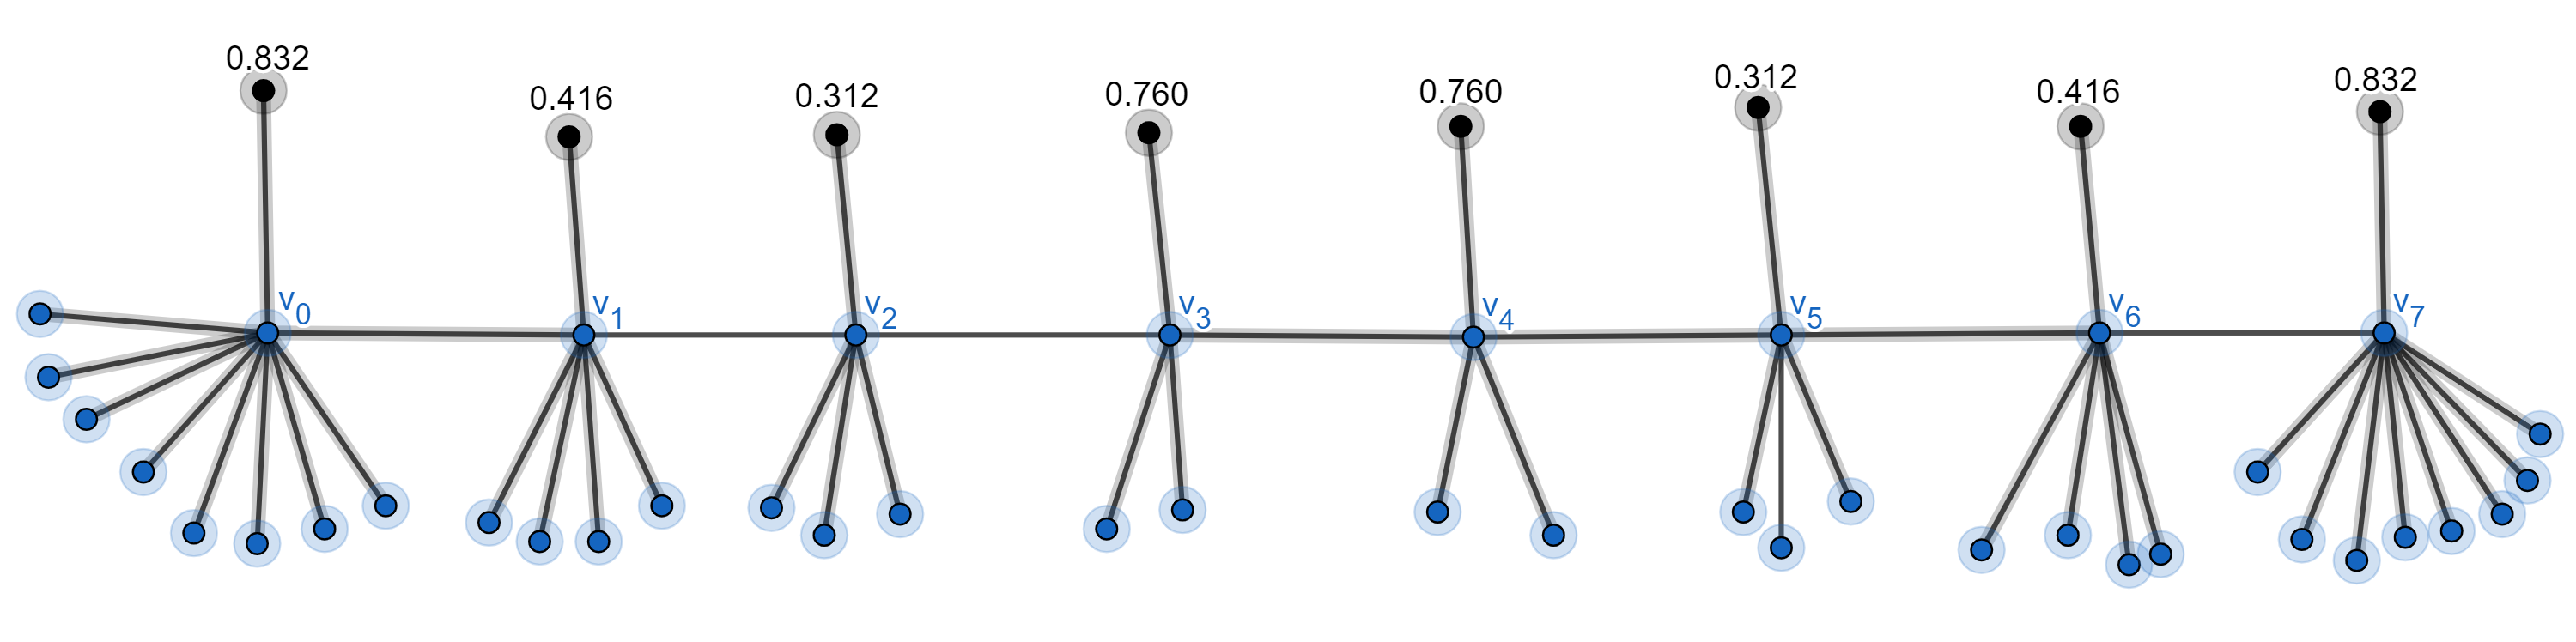
\includegraphics[scale = 0.5]{CaterpillarExample1(ConstantMults).png}
			\end{center}
		\caption{Caterpillar with larger multiplicities close to $78$, where ``close" means the quadratic terms sum to $\approx 78$.  }
		\end{figure}
		
		
		
		\end{eg}
		
		This technique can be applied so long as the choice of $b$ enables the system of equations in (\ref{Equations}) to be solved.  That is, we need to be able to find a non-negative sequence of reals $a_0, a_1, \ldots, a_n$ such that 
		$$\sum_{n \geq 0}a_nx^n = \sqrt{\sum_{n \geq 0}b_nx^n}.$$
		The trade off here is that the order of $T$ could be very large, and it is not necessarily the case that it is minimal with respect to the property of its large half of distances having the specified multiplicities.  Put another way, $T$ could have a lot of extraneous small distances.
		
		For another example, geometric progressions are also suitable choices for $b$. If $b_i = \alpha^{i}$, then a simple calculation shows that we should set $a_{d-r} = {2(d-r) \choose d-r} 4^{-(d-r)} \alpha^{d-r}$.  Here's the calculation:
		\begin{align*}
			\sum_{d-r \geq 0} \biggr(\sum_{i=0}^{d-r} a_ia_{d-r-i}\biggr)x^{d-r} &= \sum_{d-r \geq 0} \alpha^{d-r}x^{d-r}	\\
			\biggr(\sum_{d-r \geq 0} a_{d-r}x^{d-r} \biggr)^2 &= \frac{1}{1-\alpha x}	\\
			\sum_{d-r \geq 0} a_{d-r}x^{d-r} &= (1-\alpha x)^{-1/2}	\\
			&= \sum_{d-r \geq 0} {-1/2 \choose d-r}(-1)^{d-r} \alpha^{d-r}x^{d-r}	\\
			&= \sum_{d-r \geq 0}  {2(d-r) \choose d-r} 4^{-(d-r)} \alpha^{d-r}x^{d-r}.
		\end{align*}
	
	I'm hoping this is an early version of a class of techniques that allows us to construct graphs such that \textbf{*all*} (or nearly all) of its distance multiplicities closely resemble those specified.  The two main drawbacks to the above approach are (1) only half the multiplicities can be specified and (2) this can cause the order of the constructed graph to be quite large (though this varies depending on the choice of $b$), which means it might not be a minimal order construction (which would probably be a more cool thing to find).  
	
	What makes this technique work is that convolutions relate to squares of generating functions, and convolutions account for the majority of multiplicities in caterpillars with number of leaves symmetric about the center of the graph.   However, many, if not most, of the distances are not accounted for by this caterpillar construction (though it's neat that nearly half of the distance multiplicities essentially are!).  Ideally, there would be a way to get a system of maybe just less than $d$ equations so that the same number of unknowns $a_0, a_1, a_2, \ldots, a_{d-2}$ (describing number of leaves (or some other ``gadgets") to be appended to specified vertices) could be solved for, given a list of $\sim d$ specified multiplicities.  
	
	I tried playing with cycles for a bit to see if convolutions could be applied there to count multiplicities, but had no luck.  I think the convolution = square observation can only be leveraged in cases where only half the distance multiplicities are specified.  However, it might be possible to find a way to get a system of $\sim d$ equations using a caterpillar (\textit{i.e.} where we don't assume $a_i = a_{d-2-i}$).  In this case, what we would need to do is figure out how to solve the following: for each $r \in [3,d]$, we have the following system of equations:
	\begin{align}
		\mult_Q(r) = \sum_{i=0}^{d-r}a_ia_{i+r-2} = b_{r-3},
	\end{align}
	but I don't currently have any good ideas about how to work with this sum to find $a_0, a_1, \ldots, a_{d-2}$ (also, it looks like there's an extra unknown here).  Anyway, I think this section has sufficiently established that it is worth looking into this type of problem!

	\subsection{Constructing Trees That Maximize Multiplicity for a Given Distance}
	
	%Let $\mathcal{T}(k,d)$ denote the set of all trees of order $k$ and diameter $d$.  We wish to find a tree $G := G(k,d,i)$ of order $k$ and diameter $d$ that satisfies for a given distance $i \in [2,d]$ the property that $\mult_G(i) = \max_{T \in \mathcal{T}(k,d)}(\mult_T(i))$.  That is, we want $\mult_G(i)$ to be the largest possible multiplicity for distance $i$ in any tree of order $k$.
	
	%I believe that a candidate for $G$ can be a triple broom when $d \leq k/3$ and $d$ is even.  Below is a construction of $G(k,d,d)$.
	
	%Begin with an isolated vertex and append three paths of length $d/2-1$ to it. Let $v_1, v_2, v_3$ be the leaves of this tree.  Then append the remaining $k-3(d/2-1)-1$ vertices to $v_1$, $v_2$, and $v_3$ such that each has a balanced number of leaves; \textit{i.e.} $|v_i - v_j| \leq 1$ for each $i \neq j \in \{1,2,3\}$.  A computer search shows that this tree $G$ satisfies $\mult_G(d) = \max_{T \in \mathcal{T}(k,d)}(\mult_T(d))$ for all $k \leq 25$ and $d \leq \ceil{k/3}+2$.
	
	%Going forward, we will assume that $G(k,d,d)$ is the above triple broom tree.
	
	%I believe when $i$ is even, $G(k,d,i)$ can be constructed from $G(k-(d-i),d,d)$.  Construct $G(k,d,i)$ as follows: Begin with the triple broom graph $G(k-(d-i),i,i)$.  Let $v$ be a leaf, and append a path of length $d-i$ to $v$.  The resulting graph has diameter $d$, order $k$, and $\mult(i) = \mult_{G(k-(d-i),i,i)}(i) + 2(d-i)$
	
	Our goal here is to set up and state Conjecture \ref{Conjecture-TightBoundsOnEvenDistanceMultiplicities} (which I think is mostly proven below) on a tight upper bound for the multiplicities of even distances in trees of order $k$ and diameter $d$.  That is, let $\mathcal{T}(k,d)$ denote the set of all trees of order $k$ and diameter $d$, then we want to find $\max_{T \in \mathcal{T}(k,d)}(\mult_T(i))$, where $\mult_T(i)$ is the multiplicity of distance $i$ in the tree $T$.  We begin by finding the tight example for distance $d$ (when $d$ is even), and then we argue that this example can be slightly altered to maximize the multiplicity of any even distance.  What follows is a technical lemma that is necessary to prove the optimality of the construction in the diameter multiplicity case.
	
	\begin{lem}\label{Lemma-MaximizingMultiplicityInTreeTechnicalLemma}
		Let $\{a_1, a_2, \ldots, a_n\}$ be a set of positive reals such that $\sum_{i = 1}^n a_i = k - rn \geq n$, where $k, r \in \Z^+$ and $k \geq r/2$.  Then the sum $\sum_{i<j\leq n}a_ia_j$ is maximized at $f(n,k,r) = {n \choose 2}\frac{(k-rn)^2}{n^2}$
		%\frac{(n-1)(k-rn)^2}{2n}$,
		(with $a_i = \frac{k-rn}{n}$), when $n=\ceil{n_0(k,r)}$, where $n_0$ is the solution to the following cubic such that $n_0 \in [n_{\max}-1, n_{\max}]$, where $\frac{\partial}{\partial n}f(n_{\max},k,r) = 0$ and $2 \leq n_{\max} < k-rn$:
		$$n^3(2r^2) + n^2(2r^2-2kr) + n(-2kr) + k^2 = 0.$$
		%$$2(n+1)(n-1)(k-rn)^2 = 2n^2(k-r(n+1))^2.$$
	\end{lem}

	\begin{proof}[Proof Sketch]
		Observe that $\sum_{1=i<j \leq n}a_ia_j$ is maximized when $a_1 = a_2 = \cdots = a_n = \frac{k-rn}{n}$.  Thus 
		$$\sum_{i<j \leq n} a_ia_j \leq {n \choose 2}\frac{(k-rn)^2}{n^2} = \frac{(n-1)(k-rn)^2}{2n},$$
		which is the function $f(n,k,r)$ in the lemma statement.  Now we find integers $n$ that maximize $f(n,k,r)$.  Note that $f(n,k,r)$ is maximized at $n = \frac{1}{4}\big( \sqrt{\frac{8k}{r} + 1} + 1 \big) = n_{\max}$ when $k-rn \geq n$.  To find nearest integer values that maximize $f(n,k,r)$, we need to consider $f(n,k,r)$ within the interval $I$ within which $f$ is concave and $n_{\max} \in I$.   This interval $I$ is $[1,b]$ where $b$ is the unique real number satisfying $\frac{\partial^2}{\partial n^2}f(b,k,r) = 0$, whereby the concavity of $f$ fails when $n > b$.  Since $\frac{\partial^2}{\partial n^2}f(n,k,r) = r^2 - \frac{k^2}{n^3}$, $b = \frac{k^{2/3}}{r^{2/3}}$ and so $I = [1,(\tfrac{k}{r})^{2/3}]$.  Thus within this interval $I$, $f(n,k,r)$ is concave.  To find the integer(s) that maximize $f(n,k,r)$, we find $n_0$ for which $f(n_0,k,r) = f(n_0+1,k,r)$ (such an $n_0$ exists and is unique by continuity and concavity of $f$ within $I$, respectively), and then the maximal integer solution(s) will be $\{\ceil{n_0}, \floor{n_0+1}\}$.  Note that $f(n,k,r)$ has only two local extrema in $\R^+$, one local maximum at $f(n_{\max},k,r)$ in $I$ and one local minimum at $f(k/r)$ in $\R \setminus I$, so we solve the following equation for $n$ and choose the root within $I$:
		\begin{align*}
			& \frac{(n-1)(k-rn)^2}{2n} = \frac{(n)(k-r(n+1))^2}{2(n+1)}	\\
			%\Leftrightarrow &2(n+1)(n-1)(k-rn)^2 = 2n(n)(k-r(n+1))^2	\\
			\Leftrightarrow& 2(n+1)(n-1)(k-rn)^2 = 2n^2(k-r(n+1))^2	\\
			\Leftrightarrow& n^3(2r^2) + n^2(2r^2-2kr) + n(-2kr) + k^2 = 0.
		\end{align*}
	We want the solution within the interval $[x_{\max}-1,x_{\max}]$; denote this number by $n_0(k,r)$.  This $n_0(k,r)$ can be easily found for a given $k$ and $r$ using a computer solver like Sage.  Thus $f(\ceil{n_0(k,r)}, k, r)$ is the maximum of $f(n,k,r)$ over $I$ restricted to the integers. 
	
	In particular, we have the following expression for $n_0(k,r)$ [wow, simplification needed!  The root is real, so it should be possible to simplify out the $\sqrt{-1}$s somehow]:
	\begin{align*}
		n_0(k,r) = \newcommand{\Bold}[1]{\mathbf{#1}}&-\frac{1}{24} \cdot 4^{\frac{2}{3}} {\left(i \, \sqrt{3} + 1\right)} {\left(\frac{4 \, {\left(k - r\right)}^{3}}{r^{3}} + \frac{18 \, {\left(k - r\right)} k}{r^{2}} - \frac{27 \, k^{2}}{r^{2}} + \frac{3 \, \sqrt{3} k \sqrt{-\frac{8 \, k^{3} - 11 \, k^{2} r - 4 \, k r^{2} - 4 \, r^{3}}{r}}}{r^{2}}\right)}^{\frac{1}{3}} \\
		&+ \frac{4^{\frac{1}{3}} {\left(i \, \sqrt{3} - 1\right)} {\left(\frac{{\left(k - r\right)}^{2}}{r^{2}} + \frac{3 \, k}{r}\right)}}{6 \, {\left(\frac{4 \, {\left(k - r\right)}^{3}}{r^{3}} + \frac{18 \, {\left(k - r\right)} k}{r^{2}} - \frac{27 \, k^{2}}{r^{2}} + \frac{3 \, \sqrt{3} k \sqrt{-\frac{8 \, k^{3} - 11 \, k^{2} r - 4 \, k r^{2} - 4 \, r^{3}}{r}}}{r^{2}}\right)}^{\frac{1}{3}}} \\
		&+ \frac{k - r}{3 \, r}.
	\end{align*}
	This is the end of the proof.  [But like clearly I need to stare at the Sage output for $n_0(k,r)$ above for a while to figure out how to simplify it...] \qedhere
	\end{proof}


	Now back to the graph problem.  We want to find a tree of order $k$ and diameter $d$ that maximizes the multiplicity of $d$ across all such trees.  We will use Lemma \ref{Lemma-MaximizingMultiplicityInTreeTechnicalLemma} with $r = d/2-1$ and $n_0(k-1,d/2-1)$.  Since a distance $d$ is counted as a sum of products of the form $(\deg(v_i)-1)(\deg(v_j)-1)$ where $\{v_i,v_j\} \in {V(T) \choose 2}$ such that $d(v_i,v_j) = d-2$, we have for some $S \subseteq {V(T) \choose 2}$ that $\mult(d) \leq \sum_{\{v_i,v_j\} \in S}(\deg(v_i)-1)(\deg(v_j)-1)$.  By Lemma \ref{Lemma-MaximizingMultiplicityInTreeTechnicalLemma}, the largest this sum can be is when there are vertices $v_1, v_2, \ldots, v_{\ceil{n_0(k-1,d/2-1)}}$ with balanced degree and degree sum $k-1 - (d/2-1)\ceil{n_0(k-1,d/2-1)}$ each at distance $d-2$ from one another.  We construct a graph with such structure presently, denote it using $G(k,d)$, and call it a \emph{balanced-broom tree} of order $k$ and even diameter $d$.
	
	Here is the construction for a balanced-broom tree $G(k,d)$ with order $k$ and even diameter $d$.  Begin with a centre vertex $v$.  Then append $\ceil{n_0(k-1,d/2-1)}$ length $d/2-1$ paths to $v$ by identifying an end vertex of each path to $v$.  Now for the other end vertices (equivalently, the leaves of the tree built so far), call them $v_1, v_2, \ldots, v_{\ceil{n_0(k-1,d/2-1)}}$, we append $k-1-(d/2-1)\ceil{n_0(k-1,d/2-1)}$ leaves to these end vertices in a balanced way so that their degrees differ by at most one.  Let $S = \{\{v_i, v_j\}: 1 \leq i<j \leq \ceil{n_0(k-1,d/2-1)} \}$, and notice that each pair $\{v_i,v_j\} \in S$ satisfies $d(v_i,v_j) = d-2$.  Then by Lemma \ref{Lemma-MaximizingMultiplicityInTreeTechnicalLemma}, we have
	$$\sum_{\{v_i,v_j\} \in S}(\deg(v_i)-1)(\deg(v_j)-1) = \max_{\substack{T \in \mathcal{T}(k,d) \\ S' \subseteq {V(T) \choose 2} \\ \{v_i,v_j\} \in S' \\ d(v_i,v_j) = d-2}} (\deg(v_i)-1)(\deg(v_j)-1) = \max_{T \in \mathcal{T}(k,d)}(\mult_T(d)).$$
	
	That is, any tree that maximizes the multiplicity of distance $d$ must, by Lemma \ref{Lemma-MaximizingMultiplicityInTreeTechnicalLemma}, maximize the sum on the LHS; $G(k,d)$ does this, therefore $G(k,d)$ maximizes the multiplicity of $d$ across \textbf{*all*} trees of order $k$ and diameter $d$.
	
	It is straightforward to count $\mult_{G(k,d)}(d)$, so we have the following proposition.
	\begin{prop}\label{Proposition-TightDiameterCounting}
		Let $T$ be a tree of order $k$ and diameter $d$ such that $d$ is even.  Set $n_0 := n_0(k-1,d/2-1)$ as defined above and set $\ell := k-1-(d/2-1)\ceil{n_0}$.  Let $\ell = q\ceil{n_0} + s$, where $0 \leq s <\ceil{n_0}$.    Then the following bound holds with tight example $G(k,d)$:
			$$\mult_T(d) \leq {s \choose 2}\biggr\lceil{\frac{\ell}{\ceil{n_0}}}\biggr\rceil^2 + {\ceil{n_0}-s \choose 2}\biggr\lfloor{\frac{\ell}{\ceil{n_0}}}\biggr\rfloor^2 + s(\ceil{n_0}-s)\biggr\lceil{\frac{\ell}{\ceil{n_0}}}\biggr\rceil \biggr\lfloor{\frac{\ell}{\ceil{n_0}}}\biggr\rfloor.$$
		
		%$${\ceil{n_0} \choose 2}\frac{(k-1-(d/2-1)\ceil{n_0})^2}{\ceil{n_0}^2}.$$
	\end{prop}
	
	I am quite sure that a similar graph to $G(k,d)$ maximizes the multiplicity for all even distances $2 \leq i \leq d$.  The construction is simply to create a $G(k-(d-i),i)$ and then identify an end-vertex of a path of length $d-i$ to any leaf of $G(k,i)$.  This results in a graph with order $k$ and diameter $d$, which we denote by $G(k,d,i)$.  It is straightforward to see that $\mult_{G(k,d,i)}(i) = \mult_{G(k-(d-i),i)}(i) + d-i$.  I think a proof that $\mult_{G(k,d,i)}(i) = \max_{T \in \mathcal{T}(k,d)}(\mult_T(i))$ should follow from the truth of $\mult_{G(k-(d-i),i)}(i) = \max_{T \in \mathcal{T}(k-(d-i),i)}\mult_T(i)$ and showing (probably by appealing to Lemma \ref{Lemma-MaximizingMultiplicityInTreeTechnicalLemma}) that $G(k,d,i)$ is an optimal way to maximize the number of vertex pairs $\{v_i,v_j\}$ satisfying $d(v_i,v_j) = i-2$ while also having order $d$.  We just need to show that appending the path of length $d-i$ doesn't undermine optimality of $G(k,d,i)$.  I'm pretty sure that this should be easy.  Anyway, so I think the following generalization of Proposition \ref{Proposition-TightDiameterCounting} is true and our discussion thus far is at least a mostly complete proof sketch.
	
	\begin{conj}\label{Conjecture-TightBoundsOnEvenDistanceMultiplicities}
		Let $T$ be a tree of order $k$ and diameter $d$ ($d$ not necessarily even).  Let $2 \leq i \leq d$ be an even integer.  Set $n_0^{(i)} := n_0(k-(d-i)-1,i/2-1)$ and set $\ell^{(i)} := k-(d-i)-1-(i/2-1)\ceil{n_0^{(i)}}$.  Let $\ell^{(i)} = q\ceil{n_0^{(i)}} + s^{(i)}$, where $0 \leq s^{(i)} <\ceil{n_0^{(i)}}$.    Then the following bound holds with tight example $G(k,d,i)$:
		$$\mult_T(i) \leq {s^{(i)} \choose 2}\biggr\lceil{\frac{\ell^{(i)}}{\ceil{n_0^{(i)}}}}\biggr\rceil^2 + {\ceil{n_0^{(i)}}-s^{(i)} \choose 2}\biggr\lfloor{\frac{\ell^{(i)}}{\ceil{n_0^{(i)}}}}\biggr\rfloor^2 + s^{(i)}(\ceil{n_0^{(i)}}-s^{(i)})\biggr\lceil{\frac{\ell^{(i)}}{\ceil{n_0^{(i)}}}}\biggr\rceil \biggr\lfloor{\frac{\ell^{(i)}}{\ceil{n_0^{(i)}}}}\biggr\rfloor.$$
	\end{conj}
	
	If we can prove this last optimality step (showing there is no $T \in \mathcal{T}(k,d)$ such that $\mult_T(i) > \mult_{G(k,d,i)}(i)$), then we have a tight upper bound on the multiplicities of even distances in trees, which would be pretty cool!  I haven't thought much about odd distances yet -- this case seems less nice because of the lack of symmetry in the branches; but perhaps it's not too bad given the even case.  
	
	Also, I believe the \textbf{*lower bound*} problem is approachable as well, and contrary to the upper bound tight examples, which are very starry, tight examples for the lower bound should be very pathy like in long legged spiders.  Note that the lower bound tight example isn't trivially a path of length $k-1$, because $k$ can be arbitrarily larger than $d$.  So, the construction needs to have branching; but where must this branching occur, and how many branches are there?
	
	\newpage
	
	\section{Diameter Distance Removal Algorithm}
	
	\begin{prop}
		Let $T$ be a tree with distance multiset $\{1^{m_1}, 2^{m_2}, \ldots, d^{m_d}\}$.  Then there exists a sequence of graphs 
		$$T = G_d \subset G_{d-1} \subset \cdots \subset G_{2},$$
		such that for every $i \in [2,d]$, $G_i$ has distance multiset  $\{1^{m_1 + \sum_{k=i+1}^{d} m_{k}}, 2^{m_2}, 3^{m_3}, \ldots, i^{m_i}\}$.% and $j \in [2,i]$, $\mult_{G_{i}}(j) = m_j$ and $\mult_{G_{i}}(1) = m_1 + \sum_{k=0}^{i-1} m_{d-k}$.
	\end{prop}
	
	\begin{proof}
		Let $T = G_d$ be a tree with diameter $d$ and distance multiset $\{1^{m_1}, 2^{m_2}, \ldots, d^{m_d}\}$.  Let $P(T)$ be the periphery of $T$ and let $v \in P(T)$.  Observe that for every pair $\{x, y\} \subseteq P(T)$ it holds that if $d(x,y) = d$ then either $d(v,x) = d$ or $d(v,y) = d$.  This means that every diametrical path has an end vertex at distance $d$ from $v$.  Thus if $D_v = \{u \in V(T): d(v,u) = d\}$, then the graph $G_{d-1}$ produced by joining each $u \in D_v$ with the unique vertex $u'$ such that $d(v,u') = d-2$ and $d(u,u') = 2$ has diameter $d-1$.  Note we do not include multiple edges here, the edge $uu'$ can only occur once.  Since $|D_v| = m_d$, exactly $m_d$ edges are added to produce $G_{d-1}$.
		
		A very nice fact about $G_{d-1}$ is that it has distance multiset $\{1^{m_1 + m_d}, 2^{m_2}, 3^{m_3}, \ldots, (d-1)^{m_{d-1}}\}$.  This fact is explained presently: Let $T_{d-1}$ be the graph induced by all vertices with distance at most $d-2$ from $v$.  Observe that $T_{d-1}$ is a tree such that $T_{d-1} \subset T$, so the distances between vertices in $T_{d-1}$ are unchanged from those in $T$.  The distances that are changed (by adding the $m_d$ edges above) are 
		\begin{enumerate}
			\item Class 1: Those between vertices at distance exactly $d$ from $v$ and those with distance at most $d-2$ from $v$;
			\item Class 2: Let $x,y$ be at distance exactly $d$ from $v$ such that $2 \leq d(x,y) < d$ and let $P(x,y) = (x,x',\ldots, y',y)$ be the unique $(x,y)$-path in $G_d$, then the only distances that are changed when producing $G_{d-1}$ are $d(x,y) \rightarrow d(x,y) -2$, and $d(x',y) = d(x,y') = d(x,y) - 1 \rightarrow d(x,y) - 2$.
		\end{enumerate}
		  For Class 2 distances: Note that if there is a pair of vertices $x,y$ at distance $d$ from $v$ such that $2 \leq d(x,y) = t < d$ in $G_d$, then....  If $T$ is a caterpillar, then $t \leq 2$, and so $x$ and $y$ are still at distance $2$ in $G_{d-1}$ because they are not joined together in $G_{d-1}$, and $x' = y'$ where $d(x,y') = d(x',y) = 1$ is also unchanged.  
		  
		  For Class 1 distances: Each added edge $uu'$ is at the end of one of the $m_d$ diametrical paths with $v$ as end-vertex, call them $P_{u'}$.  So for each of these $m_d$ diametrical paths from $v$, for each pair of vertices $a,b \in P_{u'}$, $d(a,b)$ decreases by exactly $1$; thus if $\{1^{d}, 2^{d-1}, \ldots, d^{1}\}$ was the distance multiset of $P_{u'}$ before adding $uu'$, the distance multiset after adding $uu'$ is $\{1^{d+1}, 2^{d-1}, 3^{d-2}, \ldots, (d-1)^{2}\}$.  Of course, several of these paths must intersect, but each of them reduces the multiplicity of $d$ by $1$ and increases the multiplicity of $1$ by $1$, and all other multiplicities are left unchanged.  Since there are no other distances, we have finished proving the case for caterpillars.
		  
		  For general trees, Class 2 distances are more complicated because $t$ can be larger than $2$.  However, we can account for the Class 2 distances.  For each $t \in [3,d-1]$, define 
		  $$S_t := \{\{x,y\}\in {P(G_d) \choose 2}: d(x,v) = d(y,v) = d, d(x,y) = t\}.$$
		  Observe that $S_t$ is empty when $t$ is odd because any $(x,y)$-path intersects the $(v,x)$-path and $(v,y)$-path at exactly one point and this means that for $d(v,x) = d(v,y) = d$, $t$ must be even.  Then the multiset of Class 2 distances is 
		  $$\mathcal{C}_2 = \bigcup_{\substack{t = 4 \\ t \equiv 0 \Mod{2}}}^{d-1} \{(t-2)^{3|S_t|}, (t-1)^{-2|S_t|}, t^{-|S_t|}\}.$$
		
		Altogether, the distance multiset of $G_{d-1}$ is
		$$\{1^{m_1 + m_d}, 2^{m_2}, 3^{m_3}, \ldots, (d-1)^{m_{d-1}}\} \cup \mathcal{C}_2.$$
		
		Since $t \leq d-1$ and even, and $|S_t| \leq |P(T)|$, with each pair in $S_t$ altering $6$ distances, it follows that $\mathcal{C}_2$ alters at most $\frac{6d|P(T)|}{2} = 3d|P(T)|$ distances, which means that if the $\mathcal{C}_2$ distances were ignored, we can assume the distance multisets of $G_2$ and $G_d$ are equal up to an error of $3d|P(t)|$ distances.
		
		Another nice fact is that the set of vertices at distance at most $d-2$ from $v$ in $G_{d-1}$ induces a tree, which allows us to recursively add new edges to obtain the sequence of graphs $(G_d, G_{d-1}, \ldots, G_{2})$ satisfying the following two properties:
		\begin{enumerate}
			\item For each $i \in [3,d]$ and $j \in [2,i-1]$, it holds that $\mult_{G_i}(j) = \mult_{G_{i-1}}(j)$ and $\mult_{G_i}(1) = m_1 + \sum_{k=0}^{i} m_{d-k}$;
			\item For each $i \in [3,d]$, $G_{i} \subset G_{i-1}$.
		\end{enumerate}
		To produce $G_{i}$ from $G_{i+1}$, we join the following vertices:  for every vertex $u \in V(T)$ at distance $i+1$ from $v$, join $u$ with the unique vertex $u'$ such that $d(v,u') = i-1$ and $d(u,u') = 2$; there is such a unique vertex because the graph induced by all vertices at distance at most $i$ from $v$ in $G_{i+1}$ is a tree.  Let $T_{i+1}$ be this tree.  Note that every distance in $T_{i+1}$ is unchanged after adding the edges to form $G_i$.  The only altered distances are those involving vertices distance at most $i-1$ from $v$ and those at distance $i+1$ from $v$; for each added edge, each of these distances were reduced by $1$; these distances occur along a $(u,v)$-path such that each added edge $uu'$ causes all distances $2, 3, \ldots, i+1$ to decrease in multiplicity by exactly $1$.  Since there are $m_{i+1}$ such edges, there are $m_{i+1}$ such $(u,v)$-paths, which means that while distances do change in this process, the multiplicities $m_2, m_3, \ldots, m_i$ are unchanged with $\mult_{G_{i}}(1) = \mult_{G_{i+1}}(1) + m_{i+1}$. \qedhere
	\end{proof}
	\newpage
	
	\begin{prop}
		Let $T$ be a caterpillar with diameter $d$ and distance multiset $\{1^{m_1}, 2^{m_2}, \ldots, d^{m_d}\}$.  Let $P = (v=v_0, v_1, \ldots, v_{d})$ be a diametrical path of $T$ with end vertex $v$.  For each $j \in [1,d-1]$, let $a_i= \deg(v_i)-1$.  Then there exists a sequence of graphs
		$$T = G_d \subset G_{d-1} \subset \cdots \subset G_2,$$
		such that for each ...
		$G_{d-1}$ has distance multiset
		\begin{align*}
			&\{1^{m_1}, 2^{m_2}, \ldots, d^{m_{d}}\}	\\
			\cup &\{1^{a_{d-1}}, 2^{a_{d-1}a_{d-2}}, 3^{a_{d-1}a_{d-3}}, \ldots, (d-1)^{a_{d-1}a_1}\}	\\
			\cup &\{2^{-a_{d-1}}, 3^{-a_{d-1}a_{d-2}}, 4^{-a_{d-1}a_{d-3}}, \ldots, d^{-a_{d-1}a_1}\}	\\
			= &\{1^{m_1 + a_{d-1}}, 2^{m_2 + a_{d-1}(a_{d-2}-a_{d-1})}, 3^{m_3 + a_{d-1}(a_{d-3}-a_{d-2})}, \ldots, (d-1)^{m_{d-1} + a_{d-1}(a_1 - a_2)}\}.
		\end{align*}
		Then $G_{d-2}$ has distance multiset:
		\begin{align*}
			\{1^{m_1 + a_{d-1}+ a_{d-2}}, 2^{m_2 + a_{d-1}(a_{d-2}-a_{d-1}) + a_{d-2}(a_{d-3} - a_{d-2})}, 3^{m_3 + a_{d-1}(a_{d-3}-a_{d-2}) + a_{d-2}(a_{d-4} - a_{d-3})}, \ldots, (d-2)^{m_{d-2} + a_{d-2}(a_1 - a_2)}\}.
		\end{align*}
	\end{prop}
	
	\newpage
	
	Let $T$ be a tree and $d \in [1, \diam(T)]$.  Then the distance graph of $T$ for distance $d$ is defined to be the graph with vertex set $V(T)$ and for every $u,v \in V(T)$, $uv$ is an edge iff $d(u,v) = d$.  Denote this graph $D(T,d)$.
	
	Define a clique graph to be a graph consisting of cliques that either share a single
	
	\begin{lem}
		Let $T$ be a tree and $d \in [1, \diam(T)]$.  Then
		\begin{enumerate}
			\item If $d$ is even and does not contain an $S_{k,d/2}$ for some $k \geq 3$, then $D(T,d)$ is a clique graph.
			\item If $d$ is odd, then $D(T,d)$ is a biclique graph.
			\item If $d$ is even and contains an $S_{k,d/2}$ for some $k \geq 3$, then $D(T,d)$ is a union of clique and biclique graphs.
		\end{enumerate}
	\end{lem}
	
	
	
	\newpage
	
	\section{Distance Multiplicities Projects (June 2023)}
	
	\subsection{Crescent Sets in Graphs}
	
	A crescent set is a subset of vertices whose distances have an interval of multiplicities.  We consider graphs with order $n-1 = {k \choose 2} + (k-1)b$ where the smallest multiplicity is $b+1$ for some $k \geq 1$ and $b \geq 0$ so that the $n-1$ distances at crescent vertices can have the interval pattern.  Note the smallest multiplicity is $1$ when $b = 0$.
	
	\subsection{Minimal Tree Distance Multiset Covering}
	
	Let $\tau$ be the set of all trees of order $n$ and diameter $d$.  We wish to construct a tree $T$ with minimum order $N(n,d)$ and diameter $d$ such that the distance multiset of $T$ contains all distance multisets of trees in $\tau$.
	
	Approach: Prove sharp upper bound on multiplicities of even distances of trees.  Using this with the sharp upper bound on multiplicities of odd distances in trees from Dankelman, construct a smallest order tree that realizes these upper bounds.  That is, new results are: sharp bound for even distance multiplicities, and this construction.
	
	\begin{prop}
		A tree with order $n$ and even diameter $d$ that maximizes $\mult(d)$ is a spider with $k := k(n,d)$ legs of length $d/2 -1$ and a balanced number of leaves at the end of each leg; that is, the floor and ceiling of $\frac{n - k(d/2-1) - 1}{k} = (n-1)/k - d/2 +1$.
	\end{prop}

	\begin{proof}
		The proof is in 3 parts:
		\begin{enumerate}
			\item Show that the optimal tree contains spiders of the form $S_{k,d/2-1}$ with leaves appended to the ends of the legs.
			\item Show that the optimal tree contains exactly one $S_{k,d/2-1}$ and that the leaves are balanced across all the legs.
			\item Find the optimal number of legs $k(n,d)$ that maximizes $\mult(d)$.
		\end{enumerate}
	
		Parts 1 and 2.  Consider the distance $d$ graph of a tree $T$, denoted $D(T,d)$.  Since $d$ is even and at least $4$, $D(T,d)$ consists of only cliques and bicliques.  A $j$-clique in $D(T)$ corresponds to a spider of the form $S_{j,d/2}$ in $T$.  Bicliques in $D(T)$ correspond to length $d-2$ paths in $T$ whose end vertices are not leaves.  It is easy to see that a clique and biclique in $D(T)$ cannot intersect at more than $2$ vertices.  To maximize $\mult(d)$, we want to ensure that the independent sets in the bicliques of $D(T)$ are both large and part of many large balanced bicliques.  Since $d$ is the diameter, a part in a biclique of $D(T)$ corresponds to a set of leaves, each with the same neighbour in $T$.  Given this, we want $D(T)$ to consist of ${k \choose 2}$ bicliques, where there are exactly $k$ biclique parts with balanced size such that each biclique part is in exactly $k-1$ bicliques.  Note that the size of each biclique part is a function of $n, d,$ and $k$, where $n$ and $d$ are fixed and $k$ is variable.  So, can find a $k$ that maximizes the number of edges in $D(T,d)$, which is equal to $\mult(d)$.  The tree $T$ with this specified distance $d$ graph is a spider with $k$ (to be determined) legs, each of length $d/2 -1$, and appended to the end of each leg are a balanced number of the remaining $n - k(d/2-1)-1$ vertices.
		
		Part 3.  Find an integer $k$ that maximizes ${k \choose 2} \big(\frac{n-k(d/2-1)-1}{k} \big)^2$.
	\end{proof}

	\begin{prop}
		Let $T$ be a tree with order $n$ and odd diameter $d$.  If $T$ is a double broom, then $T$ maximizes $\mult(d)$.
	\end{prop}

	\begin{proof}
		This follows immediately when considering the distance $d$ graph of $T$.  Since $d$ is odd, $D(T,d)$ consists of only bicliques, so to maximize the number of edges in $D(T,d)$, there must be a single biclique with balanced parts.  The tree $T$ corresponding to this distance graph is a double broom with $d-2$ internal vertices and the floor and ceiling of $\frac{n-d+1}{2}$ leaves at each end.
	\end{proof}

	\begin{prop}
		Let $T$ be a tree with order $n$ and $d$ an odd integer less than $\diam(T)$.  If $T$ is a double broom with a path of length $\diam - d$ appended to a leaf, then $T$ maximizes $\mult(d)$.
	\end{prop}
	\begin{proof}
		We show that 
		\begin{align*}
			\mult(d) &\leq \biggr\lfloor{\frac{n-(d-1-(\diam-d))}{2}}\biggr\rfloor \biggr\lceil{\frac{n-(d-1-(\diam-d))}{2}}\biggr\rceil 	\\
			&= \biggr\lfloor{\frac{n-(2d-1-\diam)}{2}}\biggr\rfloor \biggr\lceil{\frac{n-(2d-1-\diam)}{2}} \biggr\rceil
		\end{align*}
		Consider the distance graph of $T$.  If $\diam - d \geq d$, then $D(T,d)$ it has a large biclique with $\diam -d-1$ $K_{1,1}$s and one $K_{\lceil{\frac{n-(2d-1-\diam)}{2}}\rceil, 1}$.  This means that
		\begin{align*}
			\mult(d) &= \lfloor{\frac{n-(2d-1-\diam)}{2}}\rfloor \lceil{\frac{n-(2d-1-\diam)}{2}} \rceil + \diam-d-1 + \lceil{\frac{n-(2d-1-\diam)}{2}}\rceil	\\
			&= \Big\lceil{\frac{n-(2d-1-\diam)}{2}} \Big\rceil^2 + \diam-d-1
		\end{align*}
		
		Alternatively, when $\diam - d < d$, there are $\diam-d$ $K_{1,1}$s and the same large biclique.  So
		$$\mult(d) = \Big\lfloor{\frac{n-(2d-1-\diam)}{2}}\Big\rfloor \Big\lceil{\frac{n-(2d-1-\diam)}{2}} \Big \rceil + \diam-d.$$
		
		The idea here is that the distance $d$ graph of a tree that maximizes $\mult(d)$ should have large balanced bicliques, and the case that maximizes the size of a large biclique is the double broom with length $d$.  Given that $T$ must contain the double broom of length $d$ and must also have diameter $\diam$, we show optimality by inductively adding vertices until the tree has the desired diameter.  Suppose $T$ is the double broom of length $d$, we wish to extend the diameter, so we must add a new vertex $u$ to a leaf $v$ (on the ceiling side).  Now for the second added vertex $w$, note that joining $w$ to $v$ increases the multiplicity of $d$ less than if we just appended $w$ to the end of the broom, thus it is sub-optimal to add vertices to a biclique in $D(T,d)$ that isn't the largest one corresponding to the double broom.  But if we added $w$ to the large biclique, then the biclique would have $x(x+2)$ edges, and the tree with diameter $d+1$ with double broom having each side of size $x+1$ has distance $d$ graph with more edges.  Thus the most optimal choice for which vertex to join with $w$ is to join $w$ with $u$.  By induction, optimality holds for each added vertex, so that a path of length $\diam - d$ is made and the resulting tree has diameter $\diam$.  This proves the exact upper bound for odd distances.
	\end{proof}
	
	
	\subsection{Classifying Winograd Families}
	
	Proving non-existence of infinite families.  Show first that there are none for small families.  Then see if can generalize.  I think the result probably follows by focusing on why the modular Winograd families only work when $k-1 \in \{\floor{n/2}-2, \floor{n/2}-1, \floor{n/2}\}$.  Idea: there must exist a largest element in an AP that is reduced modulo $n$.
	
	\subsection{Classify AP Pairs based on Multiplicity Conditions}
	
	Classify AP pairs with distinct multiplicities.  Try to extend methods from Erd\H{o}s-deep AP pairs results from Masters.  Maybe use edge weighted cycle interpretation.
	
	\subsection{Distance Max Multiplicity Games}
	
	There are 4 types of distance games on trees.  Study
	
	\newpage
	
	\section{Multiplicities as Matrix Vector Product in Trees (Nov 2023)}
	
	\begin{obs}
		Let $T$ be a tree with diameter $d$.  Then for each $x \in [3,d]$, the multiplicity of distance $x$ is given by:
		\begin{align*}
		m(x) = \sum_{\substack{\{u,v\} \in {V \choose 2} \\ d(u,v) = x-2}} (\deg(u)-1)(\deg(v)-1).
		\end{align*}
	\end{obs}

	Let $M$ be the vector of multiplicities for distances $3, 4, \ldots, d$.  Then the above observation means that each entry in $M$ can be expressed as a sum of products of degrees of the internal vertices (non-leaves) of the tree.  Let $\mathbb{T}_{d,r}$ be the set of all trees of diameter $d$ with $r$ internal vertices.  If we order the internal vertices $v_1, v_2, \ldots, v_r$ in a standardized way for all trees in $\mathbb{T}_{d,r}$, then there exists a $(d-2) \times r$ matrix $A$ such that $M = (A - \mathbf{J})(v - \mathbf{1})$, where $v$ is the standard internal vertex degree vector $[\deg(v_1), \deg(v_2), \ldots, \deg(v_r)]^T$ and $\mathbf{1}$ is the all ones vector.  Each entry in $A$ has value either $1$ or $\deg(v_i)$ for some $i \in [1,r]$.
	
	I think it would be interesting to figure out, for a fixed $d$ and $r$, what variety of matrices $A$ are possible.  Since the structure of $T$ can be completely retrieved from $A$, we can ask work exclusively with the matrix $A - \mathbf{J}$.  Indeed we have the following lemma, which shows we can obtain $A - \mathbf{J}$ by specifying only its first row:
	
	\begin{lem}
		Let $T \in \mathbb{T}_{d,r}$.  Then $A - \mathbf{J}$ is completely determined by the values in its first row.
	\end{lem}
	
	\begin{proof}
		
	\end{proof}
	
	\section{Nullstellensatz Revisited}
	
	\begin{prop}[Variation of Theorem 6.1 in \cite{alon}]\label{Prop-SubgraphNullstellensatzResult}
		Let $X$ be a set of $n$ points in a metric space, and $d$ the number of distinct distances in $\Delta(X)$.  Let $p$ be a prime number satisfying $p-1 < \tfrac{n(n-1)}{n+d}$.  Then $\mathcal{M}(X)$ contains a non-empty subgraph $U$ such that for every $u \in V(U)$, $\deg(u) \in \{kp: k \in \Z^+\}$.  %In particular, $U$ contains vertices in each part of $\mathcal{M}$, each with degree at least $p$.
	\end{prop}
	\begin{proof}
		We define a polynomial $f$ with degree $|E(\mathcal{M})|$ over $\mathbb{F}_2$, and using the fact that $a^{p-1}$ $\Mod{p}$ $\equiv 1$ for all $a \not\equiv 0 \Mod{p}$, we show the existence of the desired subgraph using the nullstellensatz directly.
		
		Define the polynomial
		$$f(x_e:e \in E(\mathcal{M})) = \prod_{v \in V(\mathcal{M})} \biggr[1 - \Big(\sum_{\substack{e \in E(\mathcal{M})\\ v \in e}}x_e \Big)^{p-1} \biggr] - \prod_{e \in E(\mathcal{M})}(1-x_e).$$
		
		The degree of $f$ is $|E(\mathcal{M})|$ because every other term has degree at most
		$$|V(\mathcal{M})| (p-1) = (n+d)(p-1) < n(n-1) = |E(\mathcal{M})|.$$
		
		Note that the max degree term of $f$, $(-1)^{|E(\mathcal{M})|+1}\prod_{e \in E(\mathcal{M})} x_e$, has a non-zero coefficient. 
		To apply the nullstellensatz, we consider solutions to $f$ of the form $(s_1,s_2,\ldots,s_{|E(\mathcal{M})|}) \in \{0,1\}^{|E(\mathcal{M})|}$ (where $t_i = 1$ for all $i \in [|E(\mathcal{M})|]$).  Thus by Lemma \ref{Lemma-CombinatorialNullstellensatz}, there exists a vector $r=(r_e:e \in E(\mathcal{M}))$ such that $f(r) \neq 0$.  By the definition of $f$, $r \neq 0$ because $f(0) = 0$, so some of its entries are $1$.  This means that the latter product in $f$ vanishes when evaluated at $r$.  The former product in $f$ can be non-zero only when $\Big(\sum_{\substack{e \in E(\mathcal{M})\\ v \in e}}r_e \Big)^{p-1} \equiv 0 \Mod{p}$.  It follows that $r$ corresponds to a subgraph $U$ of $\mathcal{M}(X)$ whose vertex degrees are congruent to $0 \Mod{p}$.  Since $r \neq 0$, there exists a vertex $u \in U$ such that $\deg(u) \in \{kp: k \in \Z^+\}$.  Note that since $U$ is a subgraph of $\mathcal{M}$, which is bipartite, the degree sums in each part need to be equal; therefore, the vertices of $U$ all have degrees being a positive multiple of $p$, and are in both parts. \qedhere
	\end{proof}
	
	
	\newpage
	\begin{thebibliography}{100}
		\bibitem{alon} Alon, N. (1999). Combinatorial Nullstellensatz. Combinatorics, Probability and Computing, 8(1-2), 7-29. doi:10.1017/S0963548398003411
	\end{thebibliography}
	
\end{document}